\documentclass[a4paper,12pt,openright,oneside]{book}
\usepackage[a4paper,margin=2in]{geometry}
\usepackage[utf8]{inputenc}
\usepackage[T1]{fontenc}
\usepackage{graphicx}
\usepackage[square,numbers,super]{natbib}
\usepackage[italian]{babel}
% le immagini vanno tutte in images/
\graphicspath{ {images/} }
\usepackage{fullpage}
\usepackage{amssymb}
\usepackage{amsthm}
\usepackage{graphics}
\usepackage{amsmath}
\usepackage{amstext}
\usepackage{lscape}
\usepackage[nottoc]{tocbibind}
\usepackage{engrec}
\usepackage{microtype}
\usepackage{enumerate}
\usepackage[hidelinks]{hyperref}
\usepackage{marginnote}
\usepackage{float}
\usepackage{setspace}
\usepackage{url}
\usepackage{pdfpages}
%\usepackage{mathptmx} % font Times New Roman (simile)
%\usepackage{amsfonts}
%\usepackage{amssymb}
\usepackage{times}
\usepackage{placeins} % per far si che le immagini rimangano nella section
\usepackage[bottom]{footmisc}
\usepackage{subcaption}
\usepackage{verbatim}




\def\UrlBreaks{\do\/\do-}


% un po' di estetica...
\usepackage{fancyhdr}
\pagestyle{fancy}
\setlength{\headsep}{0.35in}
\let\MakeUppercase\relax
\renewcommand\sectionmark[1]{}

% blocchi di codice
\usepackage{listings}
\lstset{
	breaklines=true, 
	frame=single, 
	numbers=left,
	tabsize=2,
	basicstyle=\scriptsize\small,
	showstringspaces=false
}

\frenchspacing
\thispagestyle{plain}

%% per aggiungere pagine vuote
\usepackage{afterpage}
\newcommand\myemptypage{
    \null
    \thispagestyle{empty}
    \addtocounter{page}{-1}
    \newpage
    }


\begin{document}


\includepdf[pages={1}]{Frontespizio.pdf}
\myemptypage


\cleardoublepage
\begingroup
\let\clearpage\endgroup
\null\vspace{\stretch{1}}
\frontmatter

\begin{flushright}
\begin{minipage}{5.3in}
\begin{flushright}
\begin{em}
Alla mia famiglia,
per avermi supportato psicologicamente ed economicamente in questi anni.
\\
Ai miei compagni di corso Alaa e Niccolò,
per aver reso questo percorso più sereno e me più felice.
\\
Ai miei amici,
per avermi supportato e sopportato nei momenti di difficoltà.
\\
A chiunque mi abbia aiutato e criticato,
per avermi insegnato che di fronte alle avversità non ci si deve mai arrendere.


\end{em}
\end{flushright}
\end{minipage}
\end{flushright}
\vspace{\stretch{2}} \null


\cleardoublepage
\begingroup
\let\clearpage\endgroup
\null\vspace{\stretch{1}}

\chapter*{\centering Introduzione}

Il mondo del web e del suo sviluppo ha avuto una grandissima evoluzione negli ultimi vent'anni.
Lo scopo di questa tesi è di trattare lo sviluppo web partendo dalla sua nascita, fino a raggiungere
le tecnologie più recenti utilizzate in questo ambito al fine di creare una web app.
\\
La relazione è organizzata come segue:

Nel capitolo 1 ci concentreremo sui fondamenti teorici, trattando la storia dello sviluppo web, per poi passare ai concetti base dell'architettura client server.

Nel capitolo 2 specificheremo i requisiti richiesti per lo sviluppo della web app che svilupperemo.

Nel capitolo 3 introdurremo diversi concetti generici legati alle web app.

Nel capitolo 4 andremo a descrivere le tecnologie e gli strumenti che vengono utilizzati per la creazione di una web app, trattando sia lo sviluppo front-end che lo sviluppo back-end.

Nel capitolo 5 applicheremo le tecnologie mostrate nel capitolo precedente andando a creare una web app.



\vspace{\stretch{2}} \null



\cleardoublepage

\tableofcontents
\mainmatter

\chapter{Fondamenti Teorici}

\section{La nascita del web}
Tim Berners-Lee, uno scienziato britannico, mentre lavorava al CERN nel 1989 sollevò un enorme problema che riguardava la condivisione di informazioni. Nonostante al CERN ci fosse una buona struttura gestionale per il raggiungimento degli obiettivi, Tim si rese conto che a causa dell'elevato turnover del personale, l'introduzione dei nuovi dipendenti richiedeva una grande quantità di tempo e molti dettagli tecnici dei progetti venivano persi o recuperati solo grazie ad un'indagine investigativa di emergenza.
Per risolvere questo problema, Tim propose nel marzo 1989 (Figura \ref{fig:proposta1989}) lo sviluppo del World Wide Web, la cui idea alla base era quella di creare un potente sistema informativo globale facile da utilizzare, unendo le tecnologie in costante evoluzione del web, con i data networks e gli hypertext.

La proposta fu definita \textit{"vaga ma eccitante"} dal suo capo, che nonostante lo scetticismo gli diede la possibilità di lavorarci nel settembre 1990.\\
Tim iniziò delineando le tre tecnologie che sono le fondamenta del web ancora oggi:
\begin{itemize}
\item HTML (HyperText Markup Language)
\item URI (Uniform Resource Identifier): un indirizzo che identifica ogni risorsa nel web, solitamente chiamato URL.
\item HTTP (HyperText Transfer Protocol): il protocollo che permette di recuperare le risorse all'interno del web.
\end{itemize}
Due mesi dopo, insieme all'ingegnere Robert Caillaiu, la proposta venne formalizzata delineando i concetti principali e i termini importanti sul Web (Figura \ref{fig:proposta1990}).
Alla fine del 1990 Tim Berners-Lee aveva realizzato il primo browser e Web server funzionanti.
La prima pagina web conteneva le informazioni del progetto WWW, con tutti i dettagli tecnici per la creazione di un web server e come collegarlo ad altri web server.
La creazione di questo progetto risolse il problema del recupero delle informazioni, garantendone un facile accesso.\cite{historyOfWeb}\cite{historyOfWeb2}

\begin{figure}
\centering
     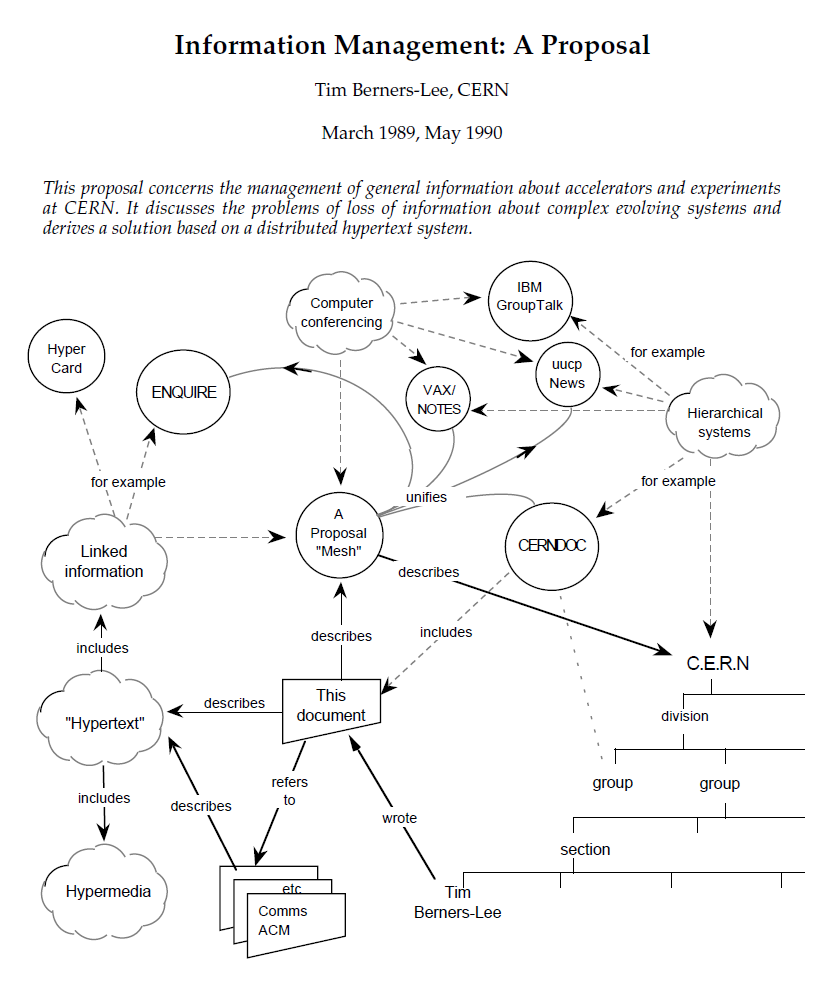
\includegraphics[width=1.0\textwidth]{images/proposta-web-1989.png}
    \caption{Prima pagina della proposta di Tim-Berners-Lee per il World Wide Web}
    \label{fig:proposta1989}
    \cite{propostaWWW1989}
    
\end{figure}

\begin{figure}
    \centering
    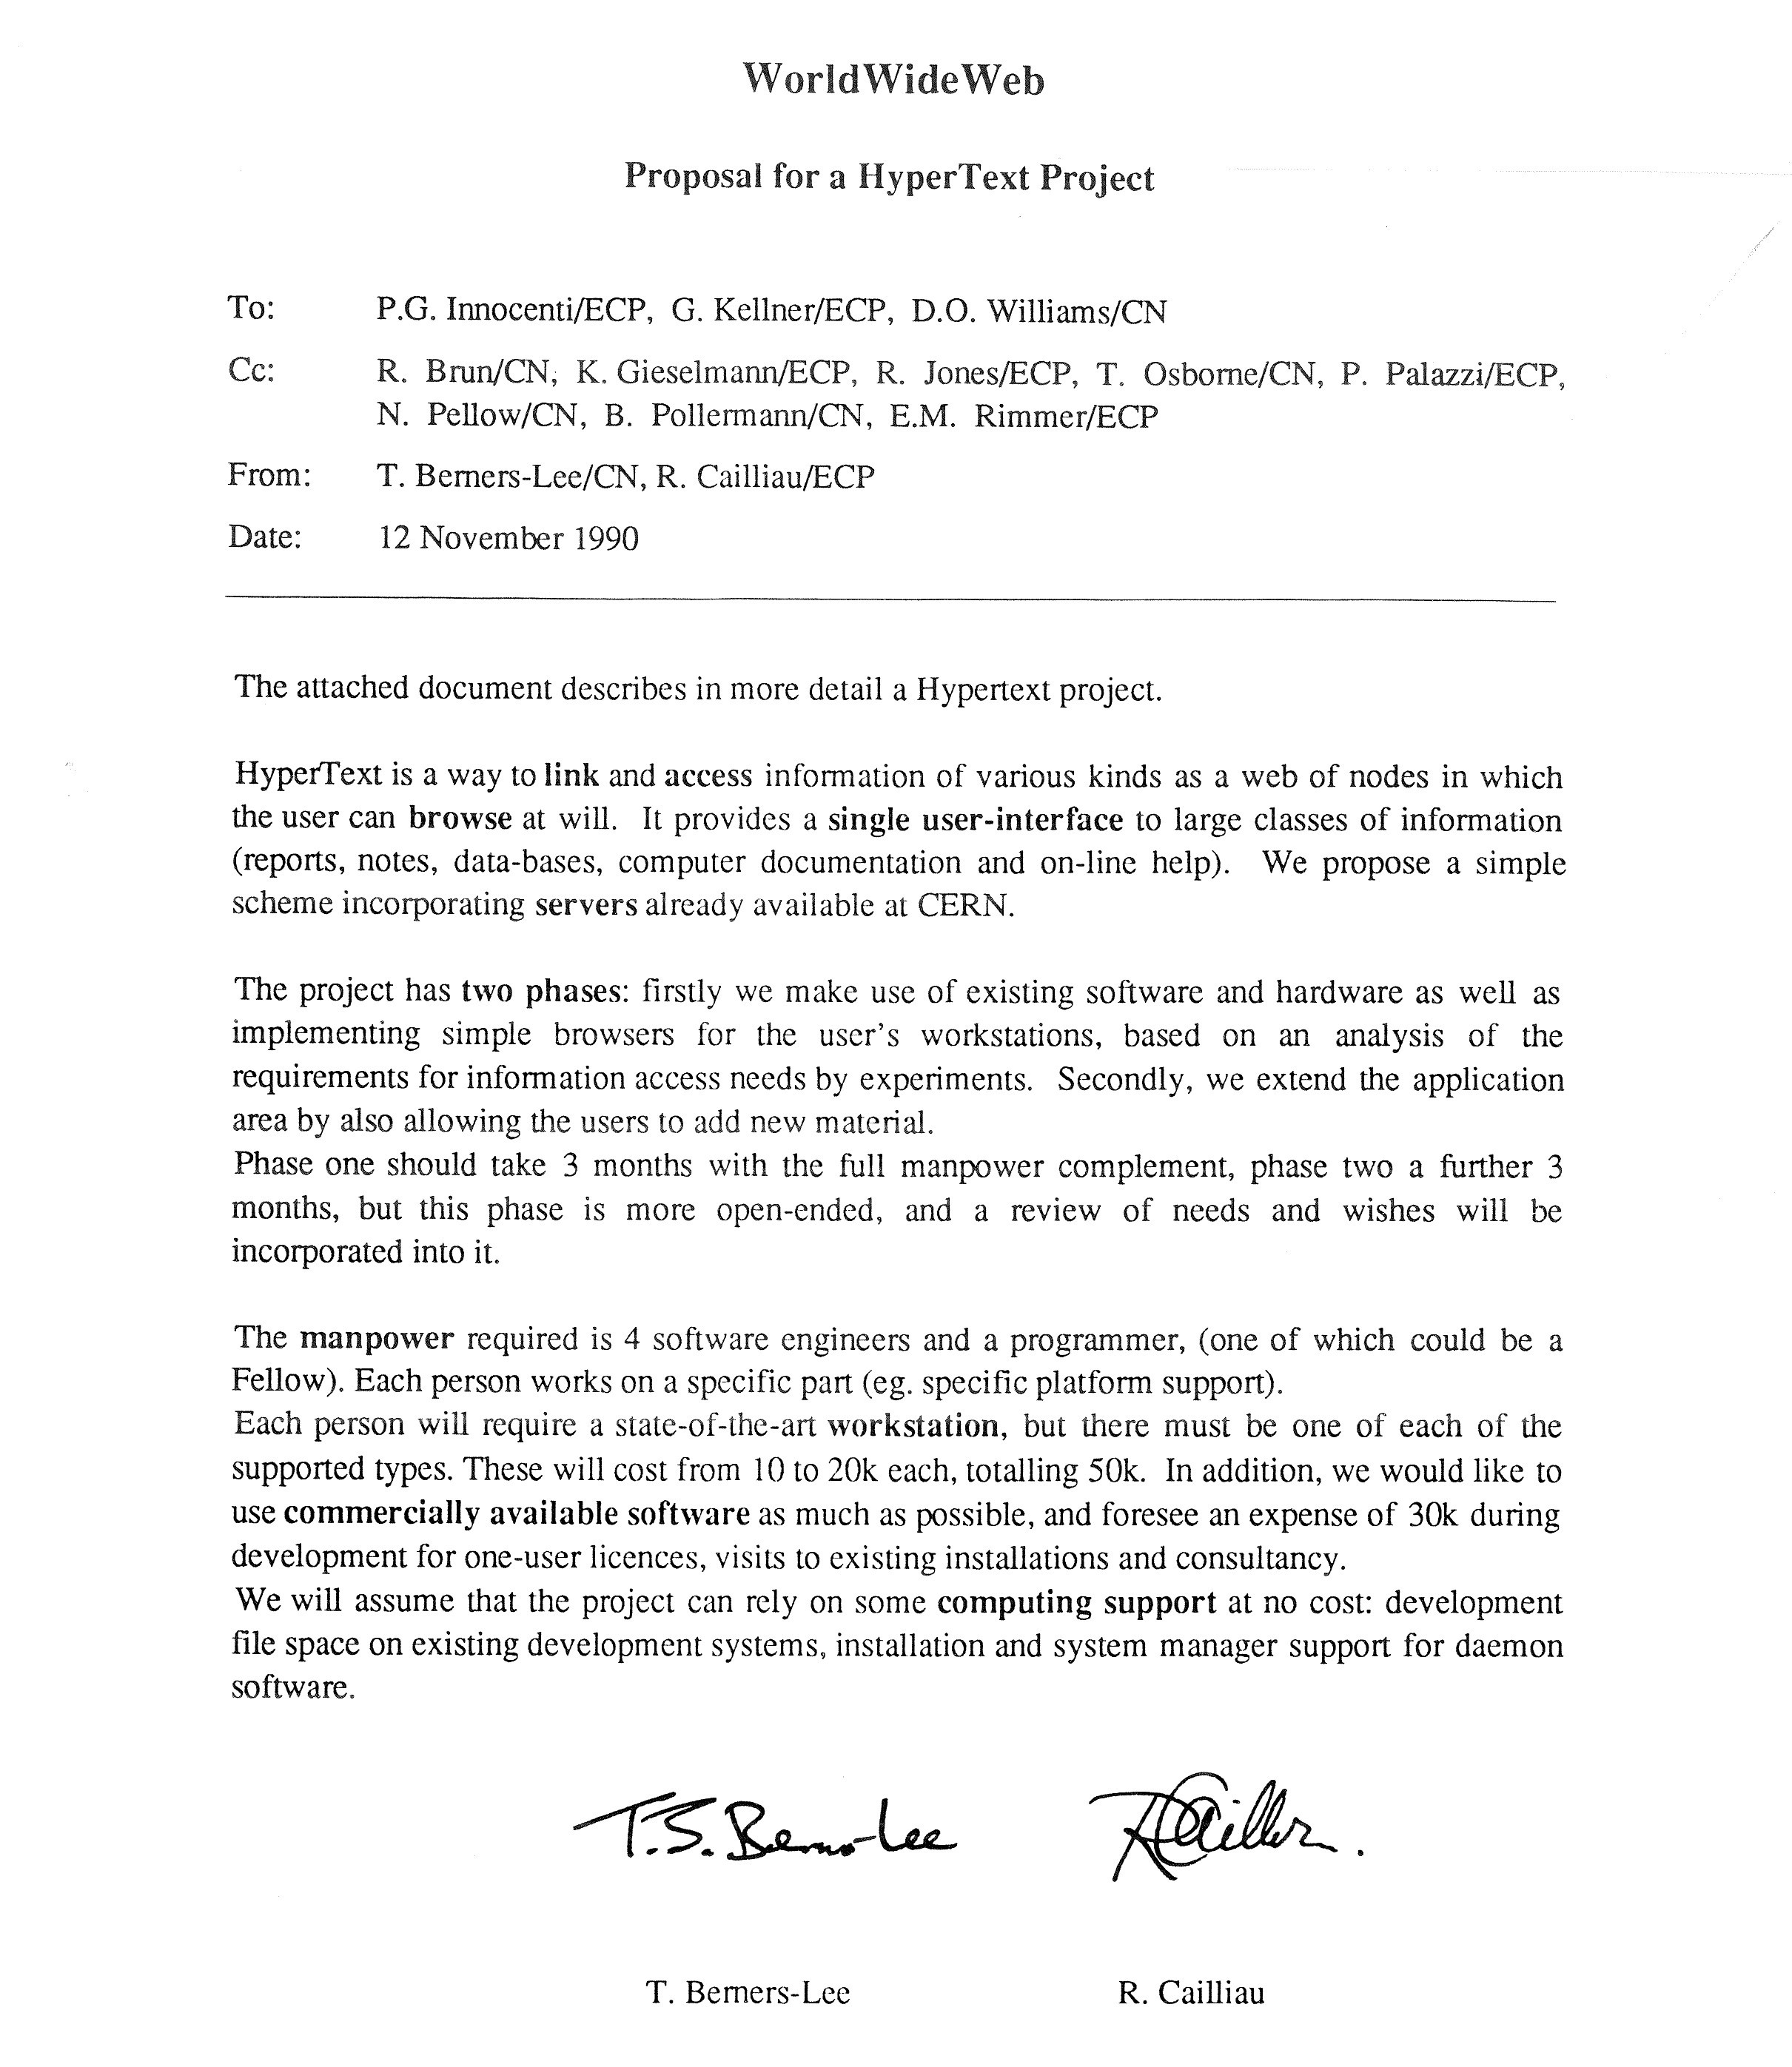
\includegraphics[width=1.0\textwidth]{images/proposta-web-1990.jpg}
    \caption{Prima pagina del documento di formalizzazione per il World Wide Web}
    \label{fig:proposta1990}
    \cite{formalizzazione1990}
\end{figure}
\FloatBarrier % per far si che ciò che scrivo successivamente appaia dopo le immagini


\section{L'evoluzione del web e la sua diffusione}
Inizialmente solo pochi utenti avevano accesso alla piattaforma informatica su cui girava il primo browser, nel quale era possibile fare ricerche solo per parole chiave dato che i motori di ricerca non esistevano ancora. Perciò si decise di sviluppare un browser più semplice che funzionava solo in modalità di linea, affinché funzionasse su ogni sistema.
Alla fine del 1991 negli Stati Uniti venne messo in rete il primo server web in un laboratorio di fisica.\\
A questo punto esistevano due tipi di browser:
\begin{itemize}
    \item La versione originale (Figura \ref{fig:browserOriginale}), la quale funzionava solo sulle macchine NeXT. \footnote{Uno dei primi computer di Steve Jobs, sul quale veniva eseguito il primo browser web.}
    \item La versione in modalità di linea (Figura \ref{fig:browserCommandLine}), la quale era più facile da installare ed eseguire su qualsiasi piattaforma, ma limitata in termini di potenza e facilità d'uso.
\end{itemize}
Date le grandi dimensioni del progetto, il team del CERN non poteva fare tutto il lavoro da solo. Perciò Berners-Lee lanciò un appello via internet al fine di trovare nuovi sviluppatori che si unissero allo sviluppo di questa rivoluzionaria tecnologia.

All'inizio del 1993 iniziarono a nascere diversi browser, che funzionavano sia in ambienti PC e Macintosh. La nascita di browser affidabili e facili da usare, comportarono una diffusione immediata del World Wide Web.

Il 1994 fu considerato \textit{"l'anno del web"} e al suo termine il Web contava 10.000 server, di cui 2.000 commerciali, e 10 milioni di utenti.\cite{historyOfWeb}
\\

\begin{figure}[h]
\begin{subfigure}{0.5\textwidth}
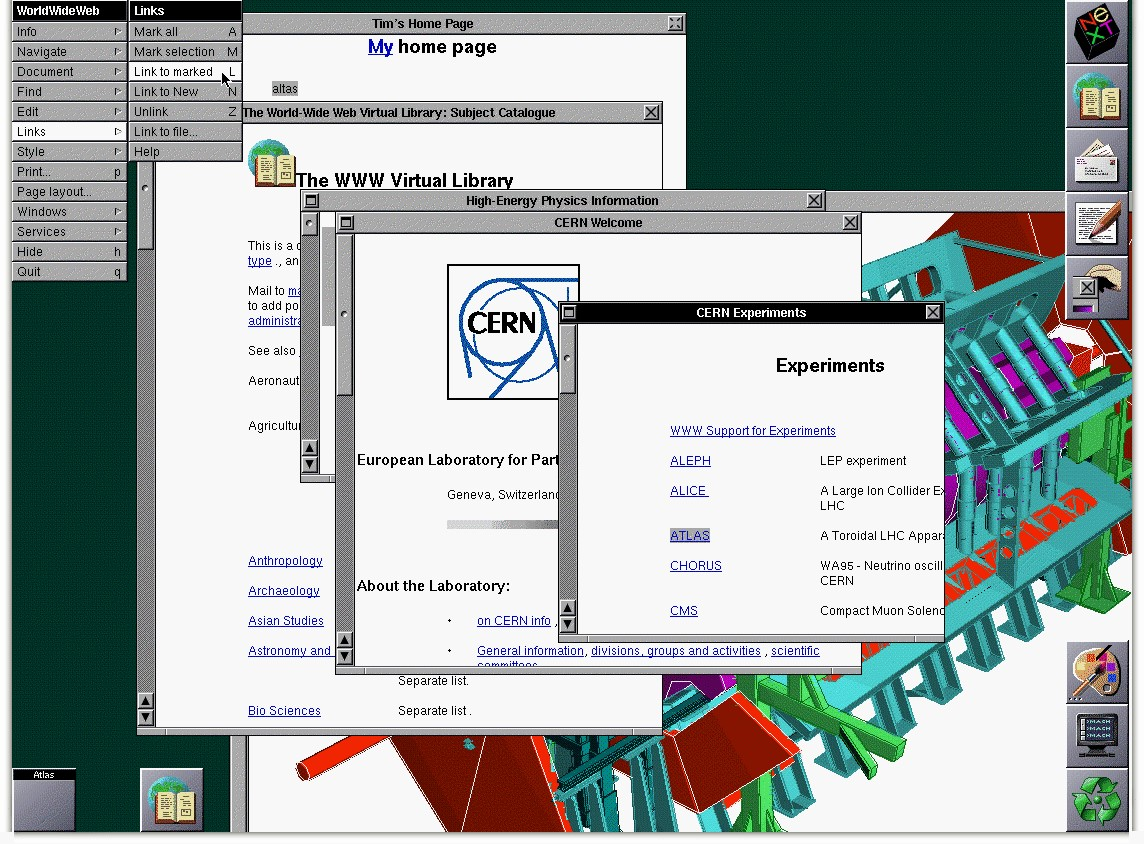
\includegraphics[width=\textwidth]{images/primo browser.jpg} 
\caption{Browser originale con interfaccia grafica}
\label{fig:browserOriginale}
\cite{primoBrowser}
\end{subfigure} \hspace*{\fill}
\begin{subfigure}{0.5\textwidth}
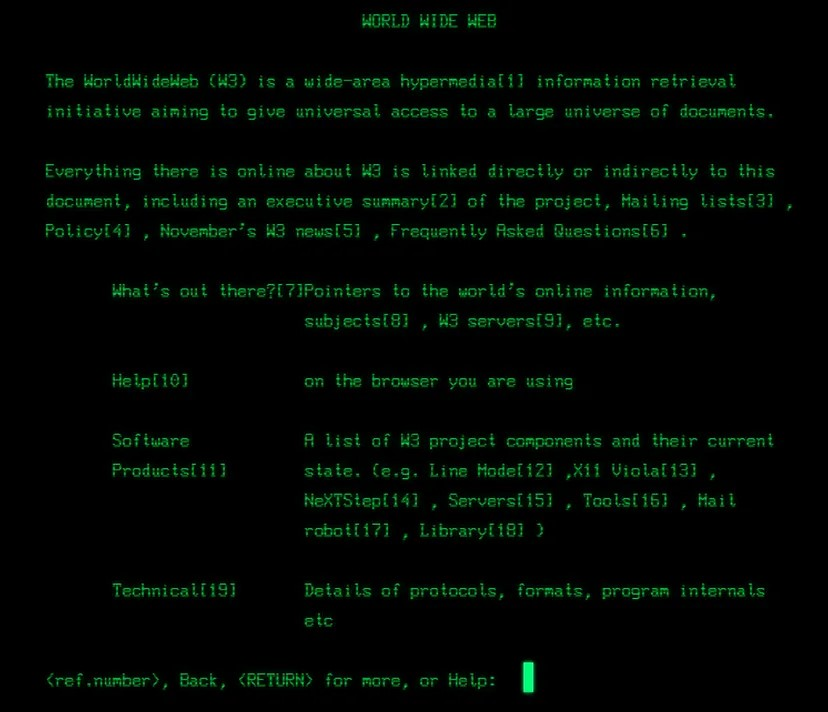
\includegraphics[width=\textwidth]{images/primo browser command line.jpg}
\caption{Browser a linea di comando}
\label{fig:browserCommandLine}
\cite{browserLineaDiComando}
\end{subfigure}

\caption{I primi due tipi di browser sviluppati nel 1991}
\label{fig:image2}
\end{figure}
\newpage
\subsection{Una tecnologia alla portata di tutti}
Gli sviluppatori al CERN decisero fin da subito che il web dovesse essere utilizzabile da tutti e che nessuno dovesse rinchiuderlo in un sistema proprietario. Per questo motivo il CERN decise di presentare una proposta, che fu subito accettata, alla commissione dell'Unione Europea al fine di formare un consorzio internazionale in collaborazione con il Massachussets Institute of Technology (MIT).

Nel 1994 Tim Berners-Lee lasciò il CERN per unirsi al MIT e fondò l'International World Wide Consortium (W3S), il quale al giorno d'oggi definisce i vari standard nello sviluppo web e di applicazioni.

Ad oggi gli standard web del W3S garantiscono un'ottimizzazione per l'interoperabilità\footnote{L'interoperabilità è, in ambito informatico, la capacità di un sistema o di un prodotto informatico di cooperare e di scambiare informazioni o servizi con altri sistemi o prodotti in maniera più o meno completa e priva di errori, con affidabilità e con ottimizzazione delle risorse.\cite{interoperabilità} \\}, la sicurezza e privacy dei dati, accessibilità e l'internazionalizzazione\footnote{L'internazionalizzazione in economia, e per estensione in informatica e altri ambiti, è il processo di adattamento di una impresa, un prodotto, un marchio, pensato e progettato per un mercato o un ambiente definito, ad altri mercati o ambienti internazionali, in modo particolare altre nazioni e culture.\cite{internazionalizzazione}}.
\\

\textit{"Web standards are blueprints or building blocks of a consistent and harmonious digitally connected world. They are implemented in browsers, blogs, search engines, and other software that power our experience on the web."}\cite{w3sStandard}

\textit{\hspace{14.2cm}- W3S}
\newpage
\section{Architettura client-server}
Un sistema client-server utilizza un'architettura nella quale un client, che è responsabile dell'interazione con l'utente e solitamente è un'interfaccia grafica di limitata complessità, si connette ad un server, il quale implementa la logica del sistema e tutte le tecniche per la gestione degli accessi, allocazione, rilascio e sicurezza delle risorse, per la fruizione di un determinato servizio, come ad esempio la condivisione di una certa risorsa.\cite{clientServer1}\cite{clientServer2}

I vantaggi di un'architettura di questo tipo sono:\cite{clientServerVantaggi}
\begin{itemize}
    \item Accessibilità dei dati: dato che il server mantiene i dati in una posizione centralizzata, più utenti possono accedere e lavorare simultaneamente sui dati garantendone una maggiore condivisione.
    \item Scalabilità: è possibile aggiornare il server ad una macchina più potente, senza cambiamenti visibili all'utente. Ciò garantisce anche la possibilità di introdurre nuove tecnologie, sia hardware che software.
    \item Integrità dei dati: il server può usufruire e fornire di servizi che garantiscono la protezione dei dati, archiviazione crittografata di file.
\end{itemize}
%\newpage
\subsection{Protocollo HTTP}
Il protocollo HTTP, il quale utilizza uno schema client-server, è una delle tecnologie alla base del web.
Quando usiamo un browser per caricare una pagina web, esso agisce come client HTTP comunicando con un server HTTP.\cite{protocolloHTTP}
\begin{figure}[h]
    \centering
    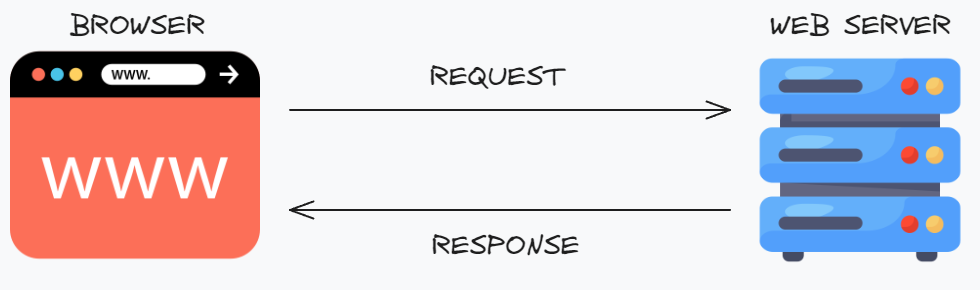
\includegraphics[width=1.0\textwidth]{images/request response.png}
    \caption{Comunicazione tra web-browser e web-server}
    \label{fig:request-response}
\end{figure}

Ad esempio, come vedremo più nello specifico nel capitolo \ref{capitolo-4}, nel momento in cui un utente vuole caricare la pagina per visualizzare i postit (Figura \ref{fig:request-response}):  
\begin{enumerate}
    \item Il browser aprirà una connessione verso il server, inviando una richiesta (request).
    \item Ricevuta la richiesta, il server si occuperà di gestire la logica di recupero dei dati richiesti, inviandoli in risposta (response) a chi ha fatto la richiesta.
    \item Il browser gestirà la risposta reindirizzando e caricando il contenuto nella pagina del sito.
\end{enumerate}
\chapter{Requisiti}
Al fine di applicare le tecnologie che tratteremo nel capitolo 4, mi è stato richiesto di sviluppare una web app.
La web app deve implementare i seguenti requisiti:
\begin{itemize} 
    \item Pagina di login: pagina in cui l'utente può autenticarsi utilizzando il proprio username e password. La password deve essere crittografata nel database utilizzando la funzione crittografica di hash Bcrypt. Inoltre ad ogni utente deve essere associato un ruolo, che viene usato per gestire i permessi di accesso alle pagine della web app. Se l'utente non ha i permessi per accedere a un determinato endpoint, quest'ultimo deve essere mandato alla pagina di accesso negato. Mentre se possiede il ruolo "EMPLOYEE" viene mandato alla home page (postit-home). (Figura \ref{fig:pagine})
    \item Homepage: pagina in cui è presente una navbar, nella quale viene mostrato il titolo della web app, l'username e il ruolo dell'utente autenticato. All'interno della navbar devono essere presenti due bottoni, uno per la creazione dei postit, l'altro per effettuare il logout.
    Inoltre sotto la navbar vengono visualizzate delle note, chiamate postit, le quali sono costituite da un titolo e descrizione. Ogni postit deve avere la possibilità di essere modificato ed eliminato.
\end{itemize}
\begin{figure}[h]
    \centering
    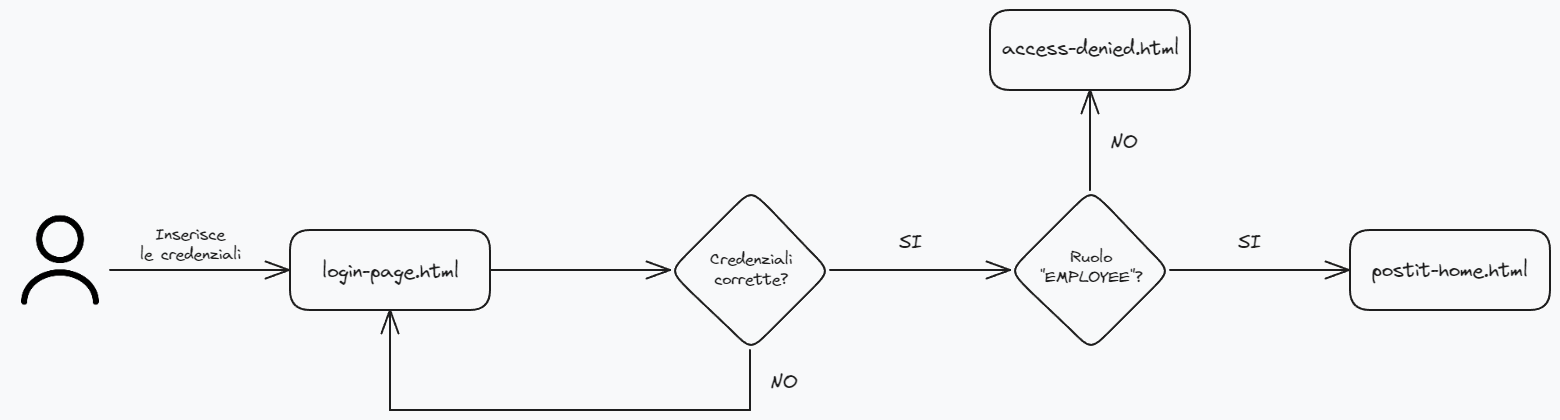
\includegraphics[width=1.0\textwidth]{images/funzionamento pagine.png}
    \caption{Pagine da implementare}
    \label{fig:pagine}
\end{figure}
\newpage
\subsubsection{Back-end}
Il back-end deve essere implementato basandosi sul pattern MVC, utilizzando il framework Spring Boot, andando a implementare:
\begin{itemize}
    \item Entità postit;
    \item Controller per login e home page;
    \item Configurazione per la gestione della sicurezza al fine di gestire l'autenticazione degli utenti e i permessi di accesso alle pagine di questi ultimi.
\end{itemize}
\subsubsection{Front-end}
Il front-end deve implementare le seguenti pagine:
\begin{itemize}
    \item login-page.html, la quale deve avere uno stile css;
    \item postit-home.html, la quale deve avere uno stile css usando il framework bootstrap;
    \item access-deniend.html
\end{itemize}
\subsubsection{Database}
I dati devono essere mantenuti all'interno di un database.
Il database, PostgreSQL, deve essere inserito in un container utilizzando l'applicativo Docker, e deve implementare le seguenti tabelle:
\begin{itemize}
    \item users
    \item ruoli
    \item postit
\end{itemize}
Al fine di recuperare i dati dal back-end e mostrarli nel front-end deve essere utilizzato il motore di template Thymeleaf.

\chapter{Concetti generici di una web app}
\section{Che cos'è una web app}
Una web app è un software applicativo eseguito su un server web, accessibile e utilizzabile da un utente tramite un browser.\cite{webApp1}
Un'applicazione web è costituita da:
\begin{itemize}
    \item Back-end: si occupa, lato server, di tutta la logica dell'applicazione, della gestione dei dati e della comunicazione con il database.
    \item Front-end: si occupa, lato client, della presentazione delle informazioni all'utente garantendo l'interazione tra utente e applicazione web.
\end{itemize}
\section{Architettura di una web app}
Una web app possiede la seguente architettura (Figura \ref{fig:funzionamento-web-app}):
\begin{enumerate}
    \item L'utente, tramite un'interfaccia dell'applicazione, invia una richiesta al server;
    \item Il client inoltra la richiesta dell'utente al server;
    \item Il server esegue l'operazione richiesta, generando i risultati dei dati richiesti;
    \item Il server invia i risultati al client, il quale si occuperà di visualizzarli all'utente.
\end{enumerate}
\begin{figure}[h]
    \centering
    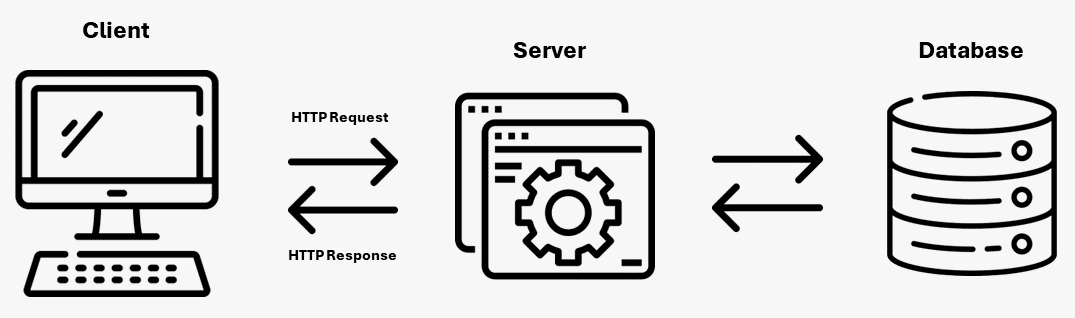
\includegraphics[width=0.9\textwidth]{images/funzionamentoWebApp.png}
    \caption{Funzionamento di un'applicazione web}
    \label{fig:funzionamento-web-app}
\end{figure}
\chapter{Architettura della soluzione - Tecnologie}
\section{Pattern MVC}
Per lo sviluppo della web app ho utilizzato il pattern MVC.
Il Model-View-Controller è un pattern utilizzato per dividere il codice in blocchi che svolgono funzionalità distinte.

Esso è costituito da tre componenti principali\cite{patternMVC} (Figura \ref{fig:pattern-mvc}):
\begin{itemize}
    \item Model: si occupa di accedere ai dati necessari alla logica implementata nell'applicazione. In particolare nella nostra web app all'interno dei model avremo la classe Postit.
    \item View: si occupano di creare l'interfaccia utilizzabile dall'utente, mostrando i dati richiesti da quest'ultimo. Nel nostro caso la view si occuperà di visualizzare, la pagina di login e tutti i postit nella homepage.
    \item Controller: si occupano di implementare la vera logica dell'applicazione utilizzando i due componenti precedenti, ricevendo gli input dell'utente, gestendo i model per la ricerca dei dati e la creazione delle view da restituire all'utente. Nel nostro caso usiamo due controller: uno per la gestione del login e uno per la gestione dei postit.
\end{itemize}
\begin{figure}[h]
    \centering
    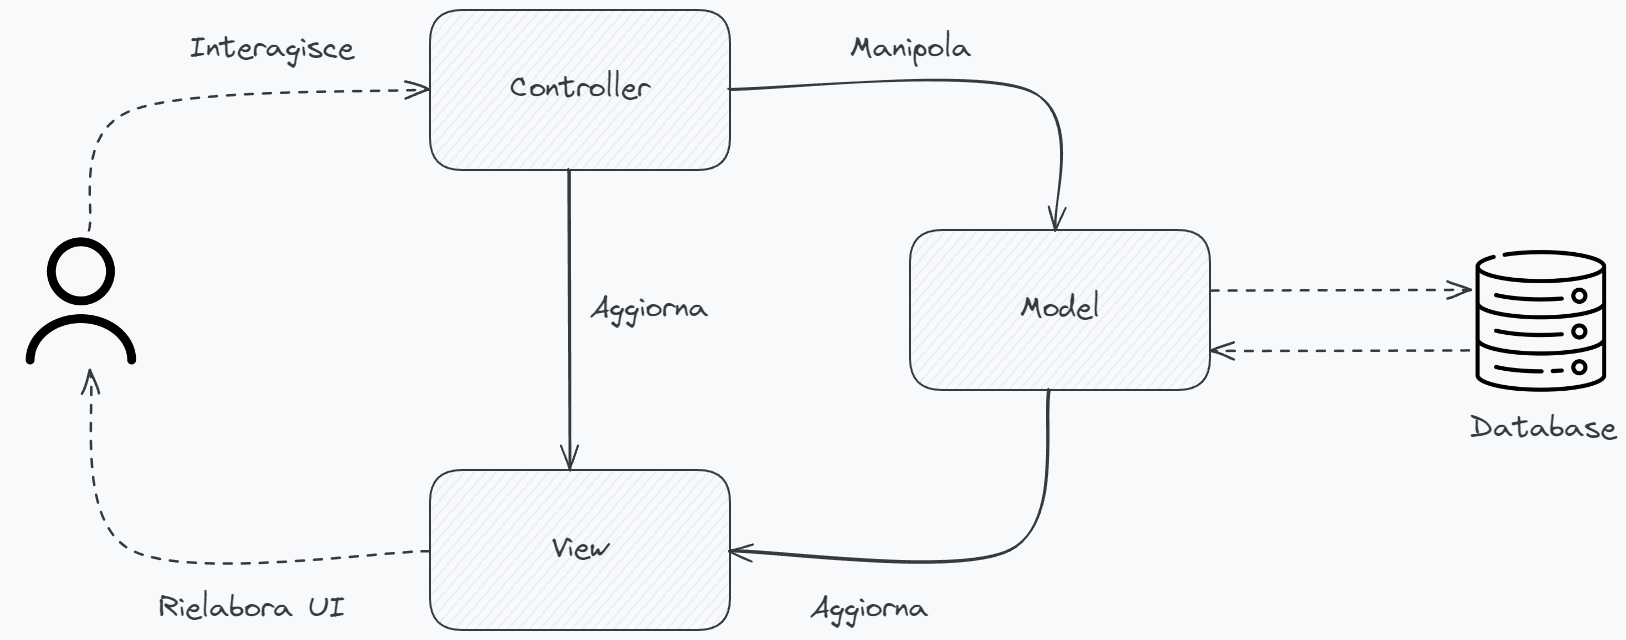
\includegraphics[width=1.0\textwidth]{images/pattern mvc.png}
    \caption{Funzionamento pattern MVC}
    \label{fig:pattern-mvc}
\end{figure}

\newpage
\section{Back-end: Tecnologie utilizzate}
Per l'implementazione del back-end ho utilizzato diverse tecnologie:
\begin{itemize}
    \item Java Spring Boot: per la gestione della logica lato server;
    \item Maven: build automation tool;
    \item Docker: per dockerizzare in un container il DB di PostgreSQL;
    \item Bcrypt: algoritmo di hashing di password;
\end{itemize}


\subsection{Spring}
Spring è un framework di Java che viene utilizzato per la creazione di applicazioni autonome, adatte ad ambienti di produzione che vengono eseguite su Java Virtual Machine.\\
Spring Boot è uno strumento che semplifica e velocizza lo sviluppo delle applicazioni web che usano Spring.
Spring fornisce una funzione di dependency-injection, che consente agli oggetti di definire le proprie dipendenze che successivamente il container Spring provvederà ad inserire. Ciò garantisce la possibilità di creare applicazioni modulari.
Dato che Spring richiede un notevole dispendio di tempo e competenze per configurare, impostare e implementare applicazioni Spring, Spring Boot riduce questo sforzo usando tre funzionalità\cite{spring}:
\begin{itemize}
    \item Configurazione automatica: le applicazioni vengono inizializzate con dipendenze preimpostate in modo tale da non doverle configurare manualmente. Grazie alla configurazione automatica, Spring Boot è in grado di configurare sia le impostazioni di Spring sia i pacchetti di terze parti. Ciò garantisce la possibilità di iniziare velocemente a sviluppare le applicazioni, riducendo errori umani.
    \item Approccio categorico per le dipendenze: Spring è in grado di scegliere i pacchetti da installare e i valori predefiniti da utilizzare evitando allo sviluppatore la perdita di tempo nel prendere tutte queste decisioni. In particolar modo durante la creazione del progetto è possibile selezionare già le dipendenze necessarie, grazie allo Spring Boot Initializr compilando semplicemente un modulo web (Figura \ref{fig:spring-initializr}). Ad esempio per la creazione di un'applicazione web è possibile selezionare "Spring Web", per garantire la sicurezza è possibile selezionare "Spring Security", ecc...
    \item Applicazioni autonome: Spring Boot consente di creare applicazioni autonome che vengono eseguite automaticamente integrando un server web come ad esempio Tomcat nell'applicazione durante il processo di inizializzazione senza dover far affidamento su un server web esterno.
\end{itemize}
\newpage
\begin{figure}[h]
    \centering
    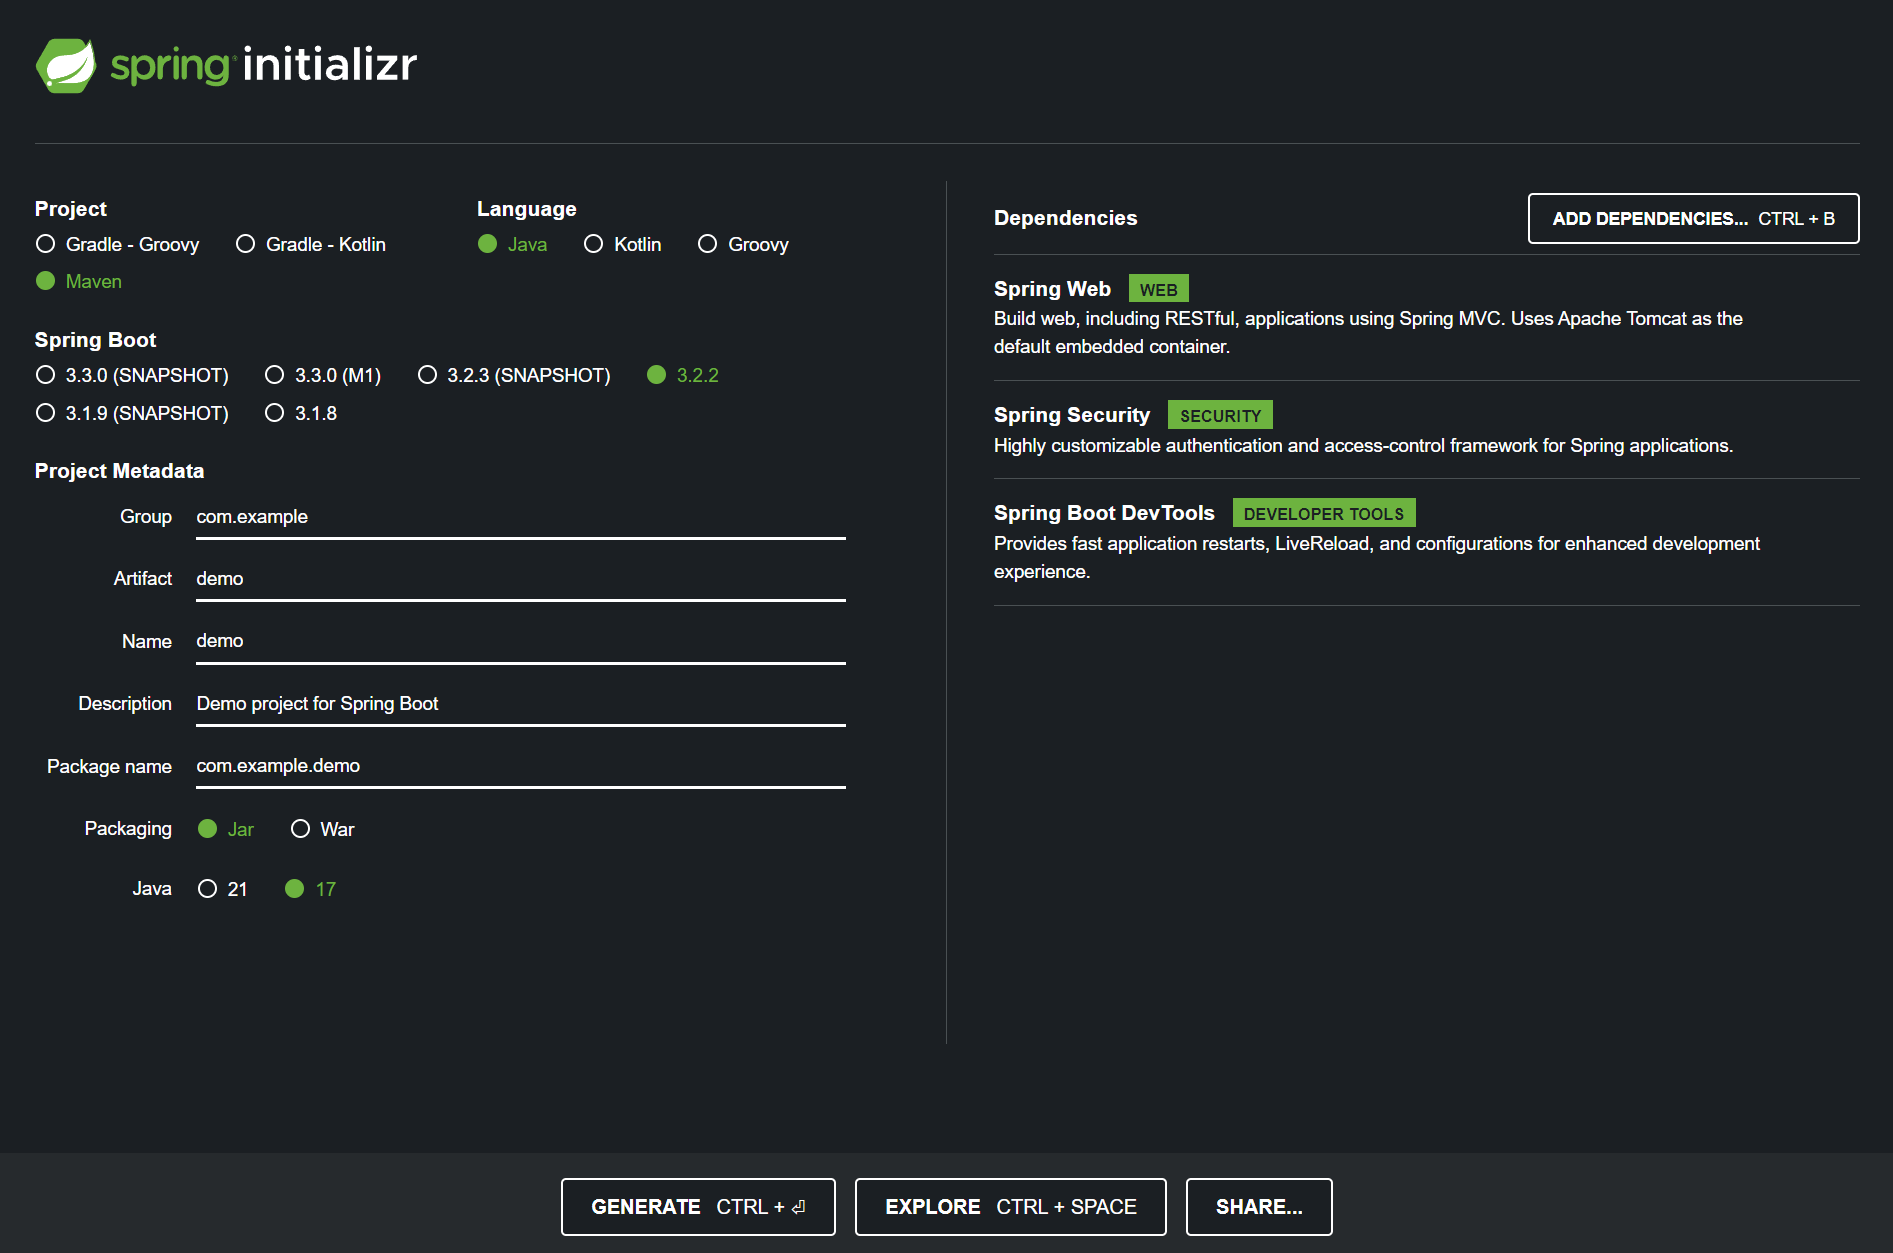
\includegraphics[width=1.0\textwidth]{images/spring initializr.png}
    \caption{Modulo web Spring Initializr}
    \label{fig:spring-initializr}
\end{figure}
\newpage

\subsection{Maven}
Apache Maven è uno strumento di automazione build utilizzato per i progetti Java.
Rende più facile gestire e mantenere grandi progetti fornendo una struttura coerente e una serie di convenzioni su come organizzare il progetto (Figura \ref{fig:organizzazione-progetto}), aiutando gli sviluppatori ad automatizzare il processo di build, test e distribuzione del software.

Una delle caratteristiche di Maven è la capacità di gestire le dipendenze, tenendo traccia di tutte le librerie e altre dipendenze di cui un progetto ha bisogno, scaricandole automaticamente.
Ciò aiuta gli sviluppatori senza il bisogno che debbano scaricare e gestire manualmente le dipendenze.\cite{maven}
\begin{figure}[h]
    \centering
    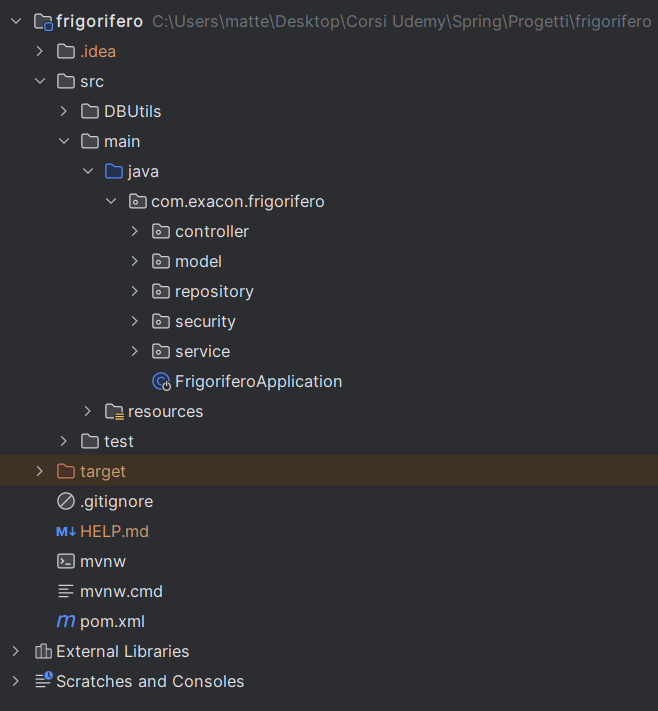
\includegraphics[scale=0.8]{images/esempio struttura progetto maven.png}
    \caption{Struttura del progetto postit-app utilizzando Maven}
    \label{fig:organizzazione-progetto}
\end{figure}

\newpage
\subsubsection{Project Object Model}
Per la gestione delle dipendenze del progetto, i plugin e la configurazione di build, Maven utilizza un file XML chiamato pom.xml (project object model).

\begin{lstlisting}[language = xml,  basicstyle=\tiny, caption={Esempio di pom.xml, nel quale sono state aggiunte le dipendenze web e database.}, captionpos=b]
<?xml version="1.0" encoding="UTF-8"?>
<project xmlns="http://maven.apache.org/POM/4.0.0" xmlns:xsi="http://www.w3.org/2001/XMLSchema-instance"
	xsi:schemaLocation="http://maven.apache.org/POM/4.0.0 https://maven.apache.org/xsd/maven-4.0.0.xsd">
	<modelVersion>4.0.0</modelVersion>
	
	<parent>
		<groupId>org.springframework.boot</groupId>
		<artifactId>spring-boot-starter-parent</artifactId>
		<version>3.2.2</version>
		<relativePath/> <!-- lookup parent from repository -->
	</parent>
	<groupId>com.example</groupId>
	<artifactId>demo</artifactId>
	<version>0.0.1-SNAPSHOT</version>
	<name>demo</name>
	<description>Demo project for Spring Boot</description>
	<properties>
		<java.version>17</java.version>
	</properties>
	
	<dependencies>
		
		<dependency>
			<groupId>org.springframework.boot</groupId>
			<artifactId>spring-boot-starter-web</artifactId>
		</dependency>

		<dependency>
			<groupId>org.postgresql</groupId>
			<artifactId>postgresql</artifactId>
			<scope>runtime</scope>
		</dependency>
		
		<dependency>
			<groupId>org.springframework.boot</groupId>
			<artifactId>spring-boot-starter-test</artifactId>
			<scope>test</scope>
		</dependency>
		
	</dependencies>

	<build>
		<plugins>
			<plugin>
				<groupId>org.springframework.boot</groupId>
				<artifactId>spring-boot-maven-plugin</artifactId>
			</plugin>
		</plugins>
	</build>

</project>

\end{lstlisting}

\newpage

\subsection{Docker}
Docker è una piattaforma open source che consente agli sviluppatori di creare, implementare, eseguire, aggiornare e gestire container, i quali sono delle unità eseguibili di software in cui viene impacchettato il codice applicativo, insieme alle sue librerie e dipendenze in modo da poter essere eseguito ovunque.
I container sono piccoli, veloci e portabili perché, diversamente da una Virtual Machine (VM), non hanno bisogno di includere un sistema operativo guest in ogni istanza, ma possono invece sfruttare le funzioni e le risorse del sistema operativo host. \cite{docker}
\subsubsection{Differenza tra container e virtual machine}
Ogni VM contiene un sistema operativo guest, una copia virtuale dell'hardware di cui il sistema operativo ha bisogno per essere eseguito, insieme a un'applicazione e alle relative librerie e dipendenze associate.
I container, a differenza delle VM, virtualizzano il sistema operativo, in modo che ogni singolo container includa solo l'applicazione e le relative librerie e dipendenze.\cite{container}
L'utilizzo dei container porta diversi vantaggi:
\begin{itemize}
    \item Leggero: i container condividono il kernel del sistema operativo della macchina, eliminando la necessità di un'istanza del sistema operativo completa per ogni applicazione e rendendo i file container piccoli e poco gravosi sulle risorse. Ciò garantisce un'esecuzione più rapida.
    \item Portabile: i container portano con loro tutte le loro dipendenze, in modo tale che il software debba essere scritto una sola volta e eseguito in diversi ambienti senza doverlo riconfigurare ogni volta.
\end{itemize}

\subsubsection{Creazione database in un container}
Per gestione del database della web app ho inserito in un container il database di PostgreSQL.
Per inserire il db in un container ho eseguito all'interno del terminale il seguente comando:
\\
\begin{lstlisting}[language=xml]
docker run --name postit-app-db ^
 -e POSTGRES_USER=utente ^
 -e POSTGRES_DB=postit-app-db ^
 -e POSTGRES_PASSWORD=password ^
 -e PGDATA=/var/lib/postgresql/data/postitData ^
 -p 5434:5432 ^
 -v C:\Docker_Data:/var/lib/postgresql/data ^
 postgres:14.1-alpine
\end{lstlisting}
\newpage
\subsubsection{Docker Desktop}
Tramite l'utilizzo dell'applicazione Docker Desktop, è possibile gestire i container ed eseguirli.
In Figura \ref{fig:docker-desktop} è possibile vedere che il container "postit-app-db" è in esecuzione.
\begin{figure}[h]
    \centering
    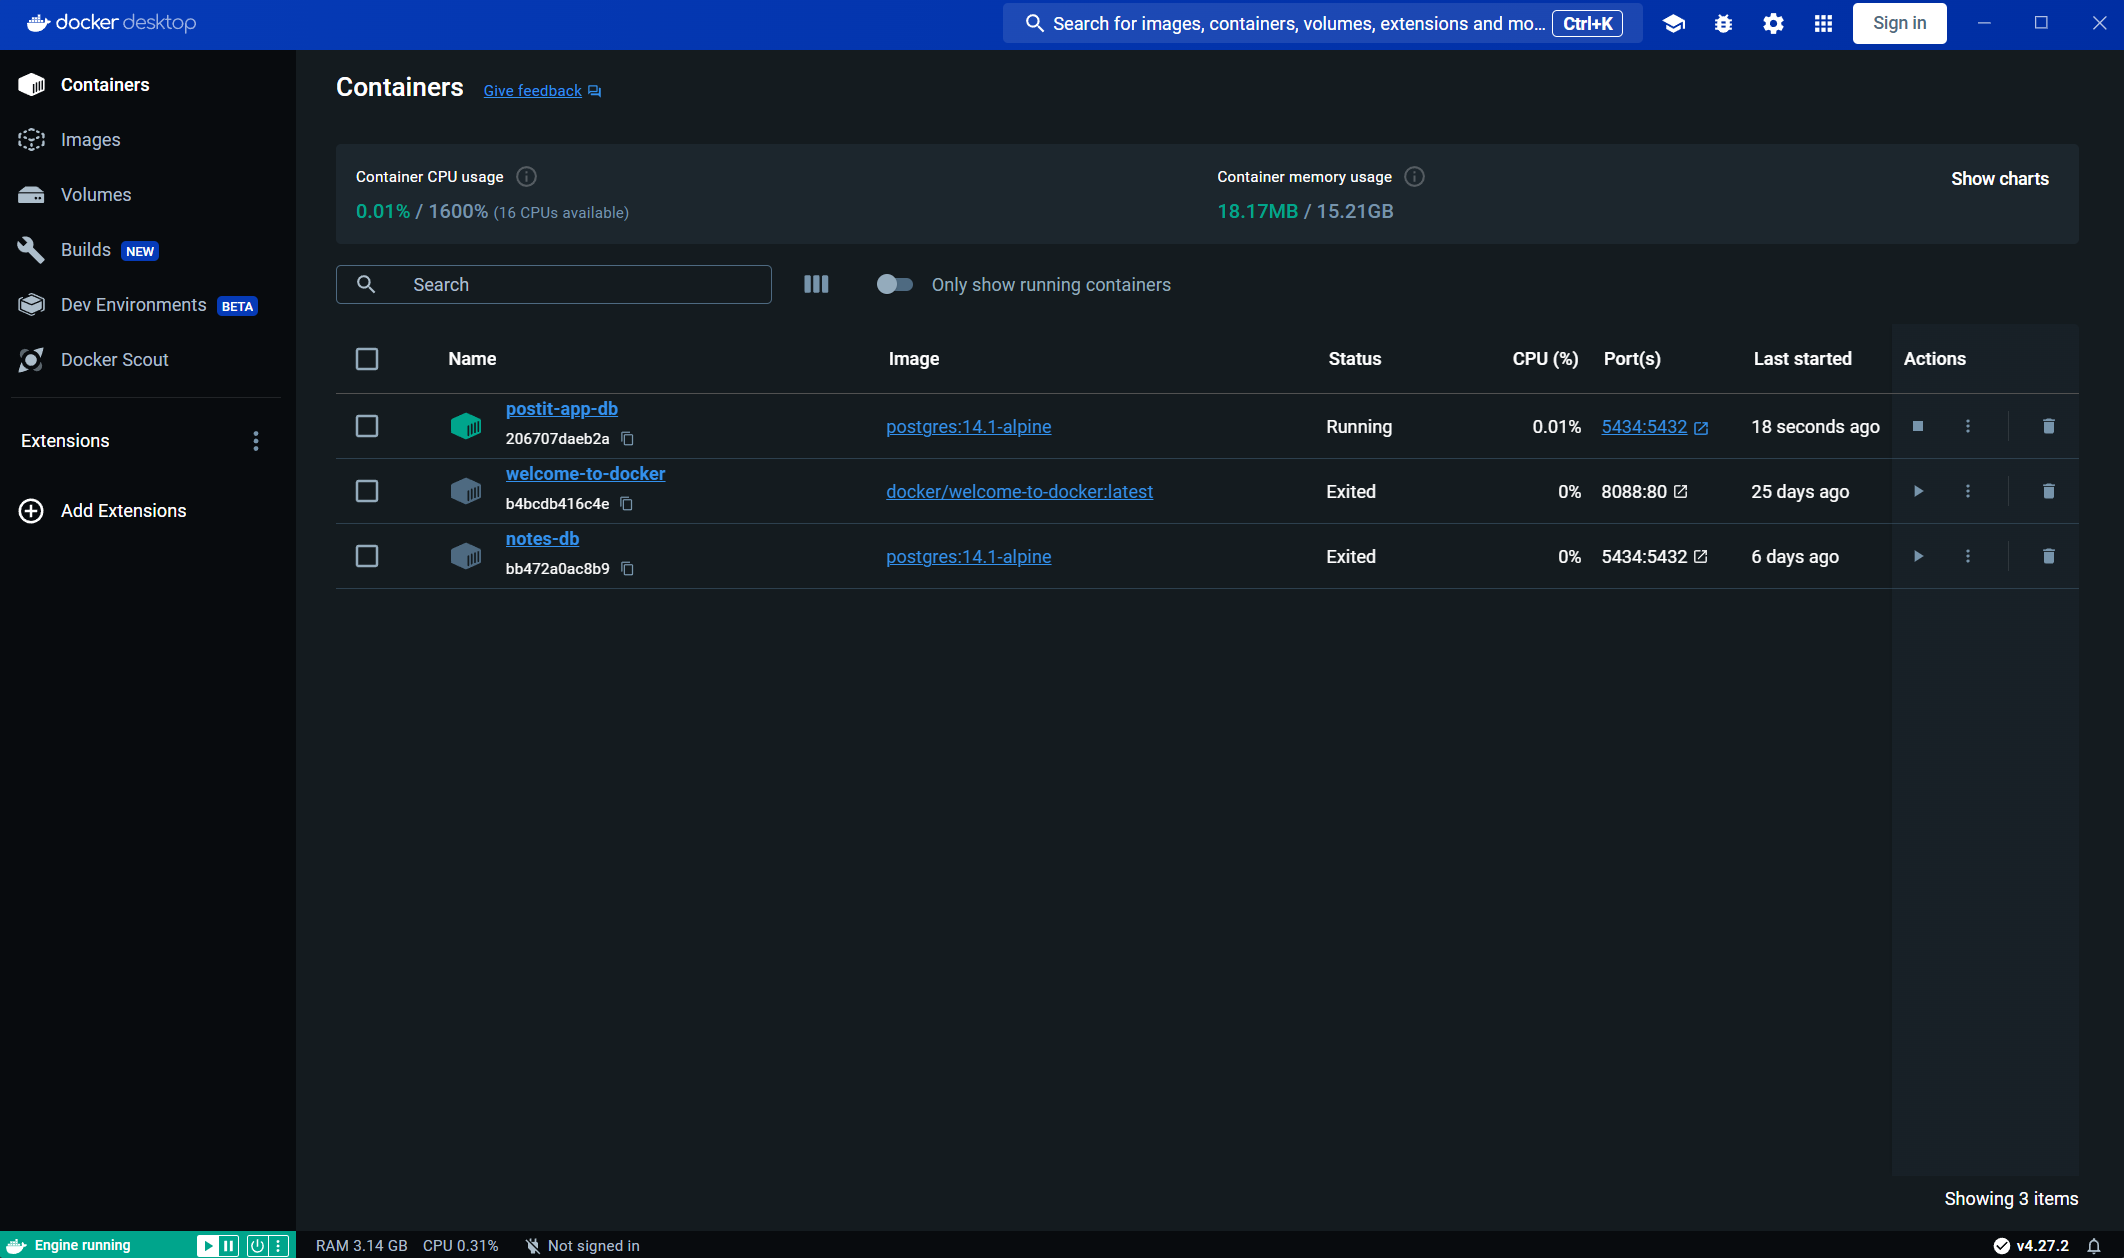
\includegraphics[width=1.0\textwidth]{images/interfaccia docker desktop.png}
    \caption{Interfaccia di Docker Desktop}
    \label{fig:docker-desktop}
\end{figure}
\newpage
\subsection{JPA - Hibernate}

\subsubsection{JPA}
Jakarta Persistent API (JPA) è un interfaccia di programmazione che consente agli sviluppatori di lavorare con i database utilizzando Java.
Viene utilizzato per recuperare e aggiornare i dati in un database.
JPA si basa sulla tecnica di programmazione ORM (Object-Relational Mapping) e può essere implementato da vari framework ORM come Hibernate (Figura \ref{fig:jpa-hibernate}) ed essere anche usato in combinazione con tecnologie Java come Spring.\cite{jpa}

\subsubsection{Hibernate}
Hibernate ORM è un framework Java utilizzato per mappare modelli di dominio orientati agli oggetti su un database relazionale (Figura \ref{fig:hibernate}).
Sostanzialmente Hibernate viene utilizzato per rendere persistenti i dati dall'ambiente Java al database.
Hibernate implementa le specifiche JPA per la persistenza dei dati\footnote{In informatica, il concetto di persistenza si riferisce alla caratteristica dei dati di un programma di sopravvivere all'esecuzione del programma stesso che li ha creati.
La persistenza si riferisce in particolare alla possibilità di far sopravvivere delle strutture dati all'esecuzione di un singolo programma. In ogni caso questa possibilità è raggiunta salvando i dati in uno storage non volatile, come su un file system o su un database. \cite{persistenza}}.\cite{hibernate}
\\
\begin{figure}[h]
    \centering
    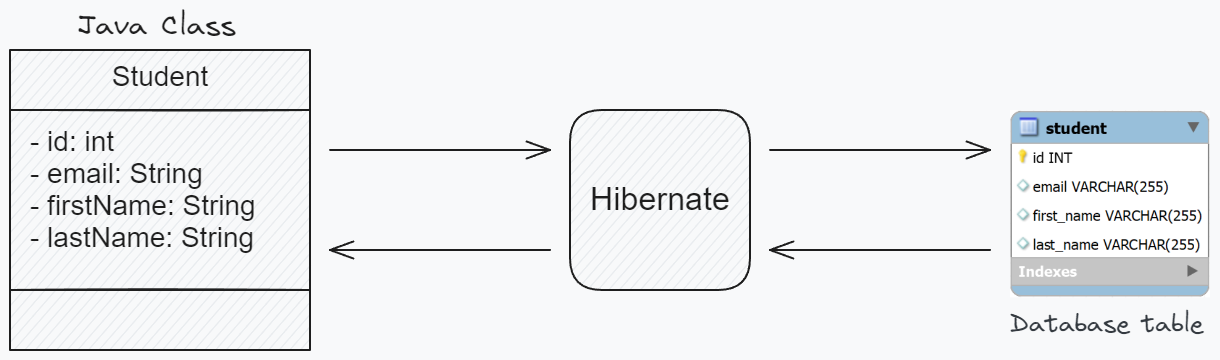
\includegraphics[width=1.0\textwidth]{images/hibernate.png}
    \caption{Funzionamento di Hibernate}
    \label{fig:hibernate}
\end{figure}

\subsubsection{JDBC}
JDBC (Java Database Connectivity) è un'API che permette di eseguire query SQL all'interno di un'applicazione Java, consentendo a queste ultime di connettersi e interrogare dei database come PostgreSQL o MySQL.\cite{jdbc}

\newpage
\subsubsection{Object-Relational Mapping}
L'Object-Relational Mapping (ORM) è una tecnica di programmazione utilizzata per memorizzare, richiamare, aggiornare ed eliminare dati da un database all'interno di programmi object-oriented solitamente scritti utilizzando linguaggi di programmazione orientata agli oggetti (OOP), come Java o C\#.
L'ORM si applica ai database relazionali, conosciuti come RDBMS (Relational Database Management System), e si occupa di convertire e tradurre tutti i dati che non potrebbero altrimenti coesistere tra database e linguaggi OOP.\cite{orm}
\\
\begin{figure}[h]
    \centering
    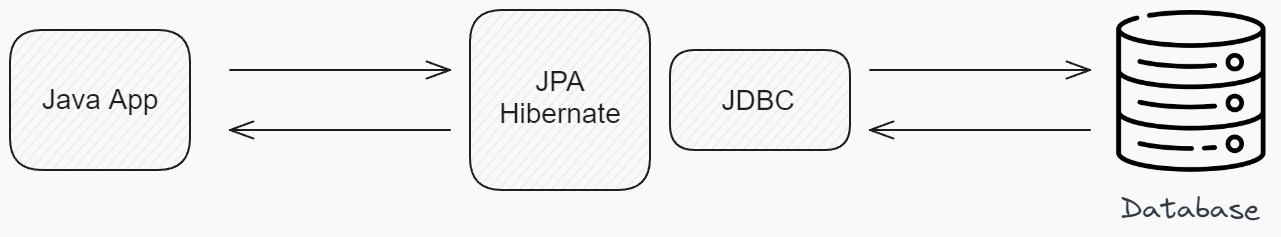
\includegraphics[width=1.0\textwidth]{images/jpa hibernate.png}
    \caption{Funzionamento di JPA con il framework ORM Hibernate.}
    \label{fig:jpa-hibernate}
\end{figure}

\subsection{Funzione crittografica di hash}
Una funzione crittografica di hash è un algoritmo che mappa dei dati di lunghezza arbitraria in una stringa binaria di dimensione fissa chiamata valore di hash, ma spesso chiamata digest.
Tale funzione di hash è progettata per essere unidirezionale (one-way), ovvero una funzione difficile da invertire: l'unico modo per ricreare i dati di input dall'output di una funzione di hash ideale, è quello di tentare una ricerca di forza bruta di possibili input per vedere se vi è un corrispondenza. \cite{funzioneCrittografica}

La funzione crittografica di hash ideale deve avere alcune proprietà fondamentali:
\begin{itemize}
    \item Deve identificare univocamente il messaggio, non è possibile che due messaggi differenti abbiano lo steso valore di hash;
    \item Deve essere deterministica, in modo che lo stesso messaggio si traduca sempre nello stesso hash;
    \item Il calcolo di un valore hash da un qualunque tipo di dato deve essere semplice e veloce;
    \item Deve essere molto difficile o quasi impossibile generare un messaggio dal suo valore hash se non provando tutti i messaggi possibili.
\end{itemize}
\newpage
\subsubsection{Bcrypt}
Bcrypt è una funzione crittografica di hash progettata per l'hashing delle password e l'archiviazione di queste ultime nel back-end delle applicazioni in modo tale da essere meno vulnerabile ad attacchi informatici.
Bcrypt esegue un processo di hasing complesso, durante il quale la password di un utente viene trasformata in un thread di caratteri a lunghezza fissa (Figura \ref{fig:bcrypt}).
Utilizza una funzione di hash unidirezionale, il che significa che una volta che la password è stata sottoposta ad hashing, non può essere ripristinata alla sua forma originale. Ogni volta che l'utente accede al proprio account, Bcrypt esegue nuovamente l'hasing della password e confronta il nuovo valore hash con la versione archiviata nella memoria del sistema per verificare se le password corrispondono. \cite{bcrypt}
\\
\begin{figure}[h]
    \centering
    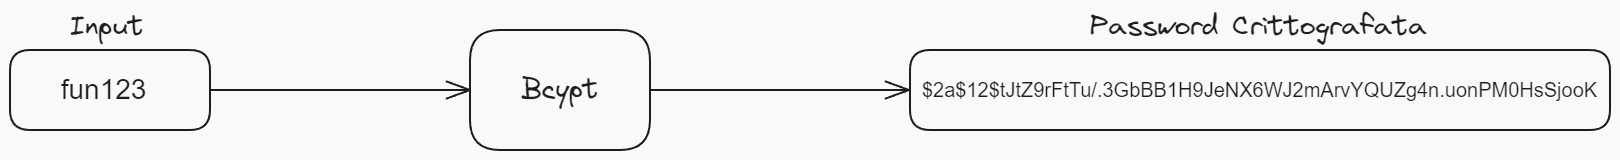
\includegraphics[width=1.0\textwidth]{images/Bcrypt.png}
    \caption{Funzionamento Bcrypt}
    \label{fig:bcrypt}
\end{figure}


\newpage
\section{Front-end: Tecnologie utilizzate}
Per l'implementazione del front-end ho utilizzato diverse tecnologie:
\begin{itemize}
    \item HTML
    \item CSS
    \item Bootstrap
    \item JavaScript
    \item Thymeleaf
\end{itemize}

\subsection{HTML}
HTML (Hypertext Markup Language) rappresenta la struttura portante delle pagine web: su questa struttura si possono aggiungere modifiche grafiche, grazie ai fogli di stile CSS ed elementi dinamici, grazie a JavaScript.
HTML è un linguaggio di markup gerarchico strutturato ad albero: esistono collegamenti gerarchici fra gli elementi, che rendono uno il genitore dell'altro ovvero il figlio.
HTML consente di descrivere semanticamente la struttura di un documento web attraverso tag, paragrafo, elenco, collegamento, citazione, o altri elementi.\cite{html}
\\
\begin{lstlisting}[language=html, basicstyle=\small, caption={Esempio di una pagina html}, captionpos=b]
<!DOCTYPE html>
<html lang="en">
<head>
    <meta charset="UTF-8">
    <meta name="viewport" content="width=device-width, initial-scale=1.0">
    <title>Document</title>
</head>
<body>

    <p>Hello World</p>
    
</body>
</html>
\end{lstlisting}
\newpage
\subsection{CSS}
CSS (Cascading Style Sheets) è un linguaggio usato per implementare lo stile di documenti scritti in un linguaggio di markup, come HTML e XML.
Con cascading in CSS si intende che i fogli di stile si applicano a cascata: quando un elemento è soggetto a diverse regole, tutte le regole sono valide, ma prevale sempre l'ultima regola. \cite{css}
Per applicare lo stile a un determinato elemento nella pagina HTML si utilizzano i selettori.

Esistono diversi tipi di selettori e vi sono delle priorità di applicazione di quest'ultimi (1 alta priorità, 6 bassa priorità):
\begin{enumerate}
    \item Dichiarazione con !important
    \item Inline style
    \item ID (\#) selector
    \item Class (.) selector, pseudo-class (:) selector
    \item Element selector
    \item Universal selector (*)
\end{enumerate}

\begin{lstlisting}[basicstyle=\small, caption={Esempio di utilizzo dei selettori usando CSS}, captionpos=b]
* {
  margin: 0;
  padding: 0;
  box-sizing: border-box;
}

p {
  font-family: sans-serif;
  color: black;
  font-size: 22px;
}

.author {
  font-style: italic;
  font-size: 18px;
}

#autor-text {
  font-size: 20px;
}

\end{lstlisting}

\subsection{Bootstrap}
Bootstrap è un framework di sviluppo web open source che permette la creazione di siti web responsive e mobile-first\footnote{Il termine Mobile First è una metodologia che promuove un modo di realizzare un’esperienza web pensata e creata nativamente per i display di dimensioni ridotte, come quelli degli smartphone e che viene progressivamente adattata e integrata per i display più grandi, come quelli dei computer desktop e delle TV.\cite{mobileFirst}}, facendo in modo che tutti gli elementi di un sito web funzionino in modo ottimale su tutte le dimensioni dello schermo.\cite{bootstrap}
Per fare ciò vengono utilizzati dei componenti, che sono recuperabili dalla documentazione.
\begin{lstlisting}[language=html, basicstyle=\small, caption={Esempio di un componente di Bootstrap (card)}, captionpos=b]
<div class="card" style="width: 18rem;">
  <img src="..." class="card-img-top" alt="...">
  <div class="card-body">
    <h5 class="card-title">Card title</h5>
    <p class="card-text">Some quick example text to build on the card title and make up the bulk of the card's content.</p>
    <a href="#" class="btn btn-primary">Go somewhere</a>
  </div>
</div>
\end{lstlisting}
\subsection{JavaScript}
JavaScript è un linguaggio di programmazione che viene utilizzato per di creare interazioni dinamiche quando si sviluppano pagine web, semplici e complesse, applicazioni, server. \cite{javascript}
JavaScript ha diversi vantaggi:
\begin{itemize}
    \item Semplicità: avere una struttura semplice rende JavaScript più facile da imparare e funziona più velocemente di altri linguaggi.
    \item Immediatezza: è eseguibile direttamente da un browser senza set-up aggiuntivi.
    \item Carico del server: operando lato client riduce le richieste inviate al server.
    \item Aggiornamenti: le community di sviluppatori aggiornano e creano nuovi framework e librerie.
\end{itemize}
\begin{lstlisting}[basicstyle=\small, caption={Esempio di script JavaScript}, captionpos=b]
document.querySelector(".btn-add").addEventListener("click", clear);

  function clear(e) {
    document.querySelector(".id-postit").value = "";
    document.querySelector(".titolo-postit").value = "";
    document.querySelector(".descrizione-postit").value = "";
  }
\end{lstlisting}
\newpage
\subsection{Thymeleaf}
Thymeleaf è un motore di template, una libreria scritta in Java, che consente agli sviluppatori di definire un modello di pagina HTML e in seguito riempirlo con i dati per generare la pagina finale.
Pertanto realizza una parte Model-View del Model-View-Controller.\cite{thymeleaf}
In particolar modo all'interno della classe Java avremo un oggetto di tipo Model, che fa da contenitore.\\
Ad esempio nella classe che fa da controller utilizziamo il model, e al suo interno possiamo inserire una lista di oggetti, a cui accederemo dalla pagina HTML per poi popolarla dinamicamente.\\
\begin{lstlisting}[language=java, basicstyle=\small, caption={Esempio di utilizzo del contenitore Model in un metodo del controller}, captionpos=b]
@RequestMapping(value = "/test")
public String showCheckbox(Model model) {
    boolean myBooleanVariable = false;
    model.addAttribute("myBooleanVariable", myBooleanVariable);
     
    return "sample-checkbox";
}
\end{lstlisting}

\begin{lstlisting}[language=html, basicstyle=\small, caption={Esempio di utilizzo di un attributo del Model all'interno della pagina HTML}, captionpos=b]
<input
 type="checkbox"
 name="myBooleanVariable"
 th:checked="${myBooleanVariable}"/>
\end{lstlisting}
\chapter{Implementazione delle tecnologie}\label{capitolo-4}
In questo capitolo ci occuperemo di applicare le tecnologie trattate nel capitolo 4, andando a sviluppare la web app "Postit-app", nella quale sarà possibile effettuare il login con il proprio account e creare, aggiornare ed eliminare delle note (postit) nella home page del sito. Ogni postit è costituito da un titolo e una descrizione.

\section{Implementazione back-end}


\subsection{Database}
Per prima cosa mi sono occupato dell'implementazione del database, e per fare ciò l'ho creato utilizzando docker eseguendo il seguente comando:
\\
\begin{lstlisting}[language=xml,basicstyle=\small, caption={Creazione del DB "postit-app-db"}, captionpos=b]
docker run --name postit-app-db ^
 -e POSTGRES_USER=utente ^
 -e POSTGRES_DB=postit-app-db ^
 -e POSTGRES_PASSWORD=password ^
 -e PGDATA=/var/lib/postgresql/data/postitData ^
 -p 5434:5432 ^
 -v C:\Docker_Data:/var/lib/postgresql/data ^
 postgres:14.1-alpine
\end{lstlisting}

Successivamente al fine di gestire i dati nel db e creare le diverse tabelle necessarie alla web app, ho utilizzato DBeaver, un'applicazione software client SQL e uno strumento di amministrazione di database.
Una volta effettuata la connessione al DB ho creato diverse tabelle:
\begin{itemize}
    \item users
    \item roles
    \item postit
\end{itemize}
\newpage
\subsubsection{Tabella users}
All'interno della tabella users ho inserito gli utenti con le loro rispettive password criptate.
\begin{lstlisting}[language=sql,basicstyle=\small, caption={Creazione tabella users}, captionpos=b]
CREATE TABLE users (
    user_id varchar(50) not null primary key,
    pw char(68) not null,
    active int not null);
\end{lstlisting}
\begin{lstlisting}[language=sql,basicstyle=\small, caption={Inserimento dati degli utenti in users}, captionpos=b]
INSERT INTO users VALUES
    ('john','{bcrypt}$2a$10$qeS0HEh7urweMojsnwNAR.vcXJeXR1UcMRZ2WcGQl9YeuspUdgF.q',1),
    ('mary','{bcrypt}$2a$10$qeS0HEh7urweMojsnwNAR.vcXJeXR1UcMRZ2WcGQl9YeuspUdgF.q',1),
    ('susan','{bcrypt}$2a$10$qeS0HEh7urweMojsnwNAR.vcXJeXR1UcMRZ2WcGQl9YeuspUdgF.q',1);
\end{lstlisting}

\subsubsection{Tabella roles}
Al fine di gestire l'accesso a determinate pagine della web app, ad ogni utente è associato un ruolo.
\begin{lstlisting}[language=sql,basicstyle=\small, caption={Creazione tabella roles}, captionpos=b]
CREATE TABLE roles (
    user_id varchar(50) references users(user_id),
    ruolo varchar(50) not null);
\end{lstlisting}
\begin{lstlisting}[language=sql,basicstyle=\small, caption={Inserimento dei ruoli nella tabella}, captionpos=b]
INSERT INTO roles VALUES
    ('john','ROLE_EMPLOYEE'),
    ('mary','ROLE_EMPLOYEE'),
    ('susan','ROLE_EMPLOYEE');
\end{lstlisting}

\subsubsection{Sequence per gestione dell'id}
Al fine di garantire un incremento dell'id numerico di ogni postit ho creato una sequence, che ho poi utilizzato nella creazione della tabella postit.
\begin{lstlisting}[language=sql,basicstyle=\small, caption={Creazione della sequence per l'id del postit}, captionpos=b]
create sequence seq_postit
increment by 1
start with 1
minvalue 1
no maxvalue;
\end{lstlisting}

\subsubsection{Tabella postit}
All'interno della tabella postit vengono salvati tutti i dati delle note e l'utente che ha creato queste ultime.
\begin{lstlisting}[language=sql,basicstyle=\small, caption={Creazione tabella postit}, captionpos=b]
CREATE TABLE postit (
    id bigint primary key default nextval ('seq_postit'),
    body varchar,
    title varchar,
    "timestamp" timestamp with time zone default current_timestamp,
    user_id varchar(50) references users(user_id));
\end{lstlisting}

\subsection{Classe Postit}
Al fine di far si che i record salvati all'interno della tabella postit, possano essere trasformati in un oggetto Java ho creato la classe Postit e per garantire questa comunicazione ho utilizzato diverse annotation:
\begin{itemize}
    \item @Entity: per far si che un oggetto Java possa interfacciarsi con il db;
    \item @Table: per associare la classe Postit alla tabella postit salvata nel db;
    \item @Column: per associare la colonna della tabella alla variabile della classe;
    \item @Id: per indicare che la variabile è un id;
    \item @SequenceGenerator: per associare la sequence del db alla variabile della classe, garantendo l'incremento automatico.
\end{itemize}
\begin{lstlisting}[language=Java,basicstyle=\tiny, caption={Classe PostIt.java}, captionpos=b]
@Entity
@Table(name = "postit")
@Getter
@Setter
@NoArgsConstructor
@AllArgsConstructor
@Builder
public class PostIt {

    @Id
    @GeneratedValue(strategy = GenerationType.SEQUENCE, generator = "seq_postit")
    @SequenceGenerator(name = "seq_postit", sequenceName = "seq_postit", allocationSize = 1)
    @Column(name = "id")
    private Long id;

    @Column(name = "body")
    private String body;

    @Column(name = "title")
    private String title;

    @Column(name = "timestamp")
    @UpdateTimestamp
    private LocalDateTime timestamp;

    @Column(name = "user_id")
    private String userId;

}

\end{lstlisting}
\newpage
\subsection{Interfaccia e classe PostitService}
In mezzo alla comunicazione tra template, controller e repository vi è la classe Service la quale si occupa di chiamare i metodi della classe repository dopo l'esecuzione di un metodo del controller.
Prima di implementare la classe PostitService ho definito un'interfaccia con al suo interno tutti i metodi utilizzati.\\
\begin{lstlisting}[language=Java,basicstyle=\small, caption={Interfaccia PostitService.java}, captionpos=b]
public interface PostitService {

    public List<PostIt> findByUser_id(String userId);
    
    public void save(PostIt thePostit);
    
    public void deleteById(Long id);

}
\end{lstlisting}
Successivamente ho implementato la classe PostitService e ho utilizzato l'annotation @Service per indicare che la classe fa da service.
All'interno di questa classe come attributo vi è l'oggetto che ci permette di riferirci alla repository e quindi a comunicare con il DB.\\
Il metodo findByUser\_id permette di cercare nel database tutti i postit che hanno come user id il valore passato come parametro, restituendo una lista di postit.\\
Il metodo save viene utilizzato per salvare un nuovo postit oppure uno modificato.\\
Il metodo deleteById permette di eliminare un postit specificando il suo id.
\begin{lstlisting}[language=Java,basicstyle=\small, caption={Classe PostitServiceImpl.java}, captionpos=b]
@Service
public class PostitServiceImpl implements PostitService {

    @Autowired
    private PostitRepository repo;

    @Override
    public List<PostIt> findByUser_id(String userId) {
        return repo.findByUserId(userId);
    }

    @Override
    public void save(PostIt thePostit) {
        repo.save(thePostit);
    }

    @Override
    public void deleteById(Long id) {
        repo.deleteById(id);
    }
}
\end{lstlisting}
\newpage
\subsection{Interfaccia PostitRepository}
L'interfaccia PostitRepository si occupa di interfacciarsi con il DB eseguendo le diverse operazioni richieste da parte del service. Per indicare che un'interfaccia o una classe è una repository ho usato l'annotation @Repository.
In Spring Boot, grazie a JPA, è possibile estendere questa interfaccia con la classe JpaRepository<PostIt, Long> la quale fornisce automaticamente tutte le operazioni CRUD, senza la necessità di dover scrivere metodi che le implementino. In particolar modo tra le parentesi angolate come primo attributo va inserita la classe che voglio utilizzare e come secondo attributo specifico il tipo dell'id della classe utilizzata, ovvero la classe PostIt.\\
\begin{lstlisting}[language=Java,basicstyle=\small, caption={Interfaccia PostitRepository che estende JpaRepository}, captionpos=b]
@Repository
public interface PostitRepository extends JpaRepository<PostIt,Long> {

    List<PostIt> findByUserId(String nome);

}
\end{lstlisting}
\subsection{Login controller}
Al fine di gestire le richieste da parte del browser per effettuare il login, ho creato la classe LoginController, nella quale ho il metodo showMyLoginPage, che una volta ricevuta la richiesta permette la visualizzazione della pagina di login.\\
Il metodo accessDenied visualizza la pagina di accesso negato, nel caso in cui un utente non possedesse i permessi per visualizzare la homepage.

In questa classe ho usato due annotation:
\begin{itemize}
    \item @Controller: per indicare che la classe è un controller.
    \item @GetMapping: per gestire la richiesta del browser. Ad esempio se nell'url è presente l'endpoint "/login", il controller si occuperà di mostrare la pagina di login eseguendo il metodo showMyLoginPage.
\end{itemize}
\newpage
\begin{lstlisting}[language=Java,basicstyle=\small, caption={Login controller}, captionpos=b]
@Controller
public class LoginController {

    @GetMapping("/login")
    public String showMyLoginPage() {

        return "login-page";
    }

    @GetMapping("/access-denied")
    public String accessDenied() {

        return "access-denied";
    }
    
}
\end{lstlisting}
\subsection{Postit controller}
La classe PostItController si occupa di gestire tutte le richieste della homepage. Nello specifico si occupa di garantire il corretto funzionamento delle funzionalità CRUD (Create, Read, Update, Delete).
Inoltre in ogni metodo viene utilizzato il PostitService, che permette di comunicare con l'interfaccia PostitRepository, che a sua volta comunica con il db.

All'interno di questa classe è possibile trovare tre metodi:
\begin{itemize}
    \item getPersonalPostits: permette di recuperare tutti i postit dell'utente corrente, inserendoli all'interno del model il quale verrà utilizzato all'interno della pagina html per visualizzare i postit.
    \item addPostit: permette di gestire la richiesta di creazione e modifica di un postit.
    \item deleteById: permette di gestire la richiesta di eliminazione di un postit.
\end{itemize}
\newpage
\begin{lstlisting}[language=Java,basicstyle=\small, caption={Postit Controller}, captionpos=b]
@Controller
@RequestMapping("/postit")
@RequiredArgsConstructor
public class PostItController {

    private final PostitService service;

    @GetMapping("/all")
    public String getPersonalPostits(Authentication authentication, Model theModel) {
        List<PostIt> personalPostits = service.findByUser_id(authentication.getName());
        PostIt p = new PostIt();
        theModel.addAttribute("postits", personalPostits);
        theModel.addAttribute("postitSingolo", p);

        return "postit-home";
    }

    @PostMapping("/add/single")
    public String addPostit(@ModelAttribute("postit") PostIt thePostit, Authentication authentication) {
        thePostit.setUserId(authentication.getName());
        service.save(thePostit);

        return "redirect:/postit/all";
    }

    @GetMapping("/delete/single")
    public String deleteById(@RequestParam("postitId") Long theId) {
        service.deleteById(theId);

        return "redirect:/postit/all";
    }

}
\end{lstlisting}
\newpage
\subsection{Configurazione login}
Per la gestione del login ho utilizzato Spring Security e ho creato una classe di configurazione al fine di configurare la corretta autenticazione di un utente.\\
Per indicare che la classe si tratta di una configurazione ho usato l'annotation @Configuration.

In questa classe sono presenti due metodi:
\begin{itemize}
    \item userDetailsManager: si occupa di gestire gli utenti all'interno del database per recuperare l'id dell'utente, la password e il ruolo associato, al fine di garantire una corretta autenticazione dell'utente.
    \item filterChain: si occupa di gestire gli accessi alle pagine statiche e template a seconda del ruolo associato. Inoltre viene gestito il login in modo tale che ad un utente, dopo essersi autenticato, venga visualizzata la homepage. Oltre al login vengono gestite le eccezioni e il logout.
    
    Nel nostro caso, un utente a cui è associato il ruolo di "EMPLOYEE" può visualizzare la homepage e accedere a tutte le funzionalità della web app. Nel caso un utente avesse un ruolo diverso da "EMPLOYEE", verrebbe mandato alla pagina di accesso negato.
\end{itemize}
\begin{lstlisting}[language=Java,basicstyle=\tiny, caption={Classe SecurityConfig.java}, captionpos=b]
@Configuration
public class SecurityConfig {

    @Bean
    public UserDetailsManager userDetailsManager(DataSource dataSource) {

        JdbcUserDetailsManager jdbcUserDetailsManager = new JdbcUserDetailsManager(dataSource);

        jdbcUserDetailsManager.setUsersByUsernameQuery(
                "SELECT user_id, pw, active FROM users WHERE user_id=?");

        jdbcUserDetailsManager.setAuthoritiesByUsernameQuery(
                "SELECT user_id, ruolo FROM roles WHERE user_id=?");

        return jdbcUserDetailsManager;
    }

    @Bean
    public SecurityFilterChain filterChain(HttpSecurity http) throws Exception {

        http.authorizeHttpRequests(configurer ->
                        configurer
                                .requestMatchers(PathRequest.toStaticResources().atCommonLocations()).permitAll()
                                .requestMatchers("/login").permitAll()
                                .requestMatchers("/error").permitAll()
                                .requestMatchers("/postit/**").hasAnyRole("EMPLOYEE")
                                .anyRequest().authenticated()
                )
                .formLogin(form ->
                        form
                                .loginPage("/login")
                                .defaultSuccessUrl("/postit/all")
                                .loginProcessingUrl("/authenticateTheUser")
                                .permitAll()
                )
                .logout(LogoutConfigurer::permitAll

                )
                .exceptionHandling(configurer ->
                        configurer.accessDeniedPage("/access-denied")
                );

        return http.build();
    }


}
\end{lstlisting}
\newpage
\section{Implementazione front-end}
\subsection{Pagina di login}
All'interno della login-page.html è presente un form in cui l'utente può inserire l'username e la password per autenticarsi.
Se le credenziali di accesso sono corrette spring security si occuperà di mandare l'utente alla homepage. In caso contrario viene visualizzato un messaggio di errore.
\begin{lstlisting}[language=html,basicstyle=\tiny, caption={login-page.html}, captionpos=b]
<!DOCTYPE html>
<html lang="en" xmlns:th="http://www.thymeleaf.org">
  <head>
    <meta charset="UTF-8" />
    <meta name="viewport" content="width=device-width, initial-scale=1.0" />
    <link
      rel="stylesheet"
      href="https://cdnjs.cloudflare.com/ajax/libs/font-awesome/6.4.2/css/all.min.css"
    />
    <link th:href="@{/css/login.css}" type="text/css" rel="stylesheet" />

    <title>Login Page</title>
  </head>

  <body>
    <div class="container1" id="container">
      <div class="form-container sign-in">
        <form action="#" th:action="@{/authenticateTheUser}" method="POST">
          <h1>Sign In</h1>

          <div>
            <!-- Check for login error -->
            <div th:if="${param.error}">
              <div>
                <p class="invalid-username">Invalid username or password.</p>
              </div>
            </div>

            <div th:if="${param.logout}">
              <div class="alert alert-success col-xs-offset-1 col-xs-10">
                <p class="logout">You have been logged out.</p>
              </div>
            </div>
          </div>

          <input type="text" name="username" placeholder="Username" />
          <input type="password" name="password" placeholder="Password" />
          <button>Sign In</button>
        </form>
      </div>
      <div class="toggle-container">
        <div class="toggle">
          <div class="toggle-panel toggle-right">
            <h1>Welcome to the Postit App</h1>
            <p>Sign In to se your personal postits!</p>
          </div>
        </div>
      </div>
    </div>
  </body>
</html>

\end{lstlisting}
\newpage
\subsection{Homepage}
Nella pagina postit-home.html è presente una navbar in cui viene visualizzato il nome dell'utente e il suo ruolo. Inoltre sono presenti i bottoni che permettono di creare un nuovo postit ed effettuare il logout.
Al di sotto della navbar vengono visualizzati i postit, i quali hanno un titolo, una descrizione e i bottoni che permettono di modificare o eliminare il postit selezionato.
I postit vengono visualizzati grazie all'utilizzo di un foreach, il quale scorre la lista di postit creati dall'utente e per ognuno crea una card nella quale vengono inseriti i corrispettivi dati.
La lista di postit creati dall'utente viene recuperata grazie all'utilizzo del contenitore model di Thymeleaf.
\begin{lstlisting}[language=html,basicstyle=\tiny, caption={postit-home.html}, captionpos=b]
<!DOCTYPE html>
<html
  lang="en"
  xmlns:th="http://www.thymeleaf.org"
  xmlns:sec="http://www.thymeleaf.org/extras/spring-security"
>
  <head>
    <meta charset="UTF-8" />

    <!-- bootstrap -->
    <link
      href="https://cdn.jsdelivr.net/npm/bootstrap@5.3.2/dist/css/bootstrap.min.css"
      rel="stylesheet"
      integrity="sha384-T3c6CoIi6uLrA9TneNEoa7RxnatzjcDSCmG1MXxSR1GAsXEV/Dwwykc2MPK8M2HN"
      crossorigin="anonymous"
    />
    <link
      rel="stylesheet"
      href="https://cdnjs.cloudflare.com/ajax/libs/font-awesome/6.4.2/css/all.min.css"
    />
    <link
      rel="stylesheet"
      href="https://cdnjs.cloudflare.com/ajax/libs/font-awesome/6.4.2/css/all.min.css"
    />
    <link th:href="@{/css/home.css}" type="text/css" rel="stylesheet" />

    <title>Postit App</title>
  </head>

  <body>
    <!-- navbar start -->
    <nav class="navbar navbar-expand-lg bg-body-tertiary naviga">
      <div class="container-fluid">
        <a class="navbar-brand titolo-app" href="#">Postit App</a>
        <div class="container d-flex align-items-center ms-3 ps-5">
          <p class="m-0 utente">
            Hello,
            <span class="utente" sec:authentication="principal.username"></span
            >!
          </p>
          <p class="ps-2 m-0 utente">
            Your role is:
            <span
              class="utente"
              sec:authentication="principal.authorities"
            ></span>
          </p>
        </div>

        <div
          class="container d-flex align-items-center m-0 justify-content-end"
        >
          <!-- Button trigger modal -->
          <button
            type="button"
            class="btn btn-add"
            data-bs-toggle="modal"
            data-bs-target="#exampleModal"
          >
            ADD POSTIT
          </button>

          <form action="#" th:action="@{/logout}" method="POST" class="ps-3">
            <button type="submit" class="btn btn-logout">Logout</button>
          </form>
        </div>

        <!-- Modal -->
        <div
          class="modal fade modale"
          id="exampleModal"
          tabindex="-1"
          aria-labelledby="exampleModalLabel"
          aria-hidden="true"
        >
          <div class="modal-dialog">
            <div class="modal-content">
              <div class="modal-header">
                <h1 class="modal-title fs-5" id="exampleModalLabel">
                  Postit Modal
                </h1>
                <button
                  type="button"
                  class="btn-close"
                  data-bs-dismiss="modal"
                  aria-label="Close"
                ></button>
              </div>
              <div class="modal-body">
                <form
                  id="postit-form"
                  action="#"
                  th:action="@{/postit/add/single}"
                  th:object="${postitSingolo}"
                  method="post"
                >
                  <div class="mb-3">
                    <label class="form-label">Title</label>

                    <input
                      type="hidden"
                      class="form-control id-postit"
                      th:field="*{id}"
                    />

                    <input
                      type="text"
                      class="form-control titolo-postit"
                      th:field="*{title}"
                    />
                  </div>
                  <div class="mb-3">
                    <label class="form-label">Body</label>
                    <input
                      type="text"
                      class="form-control descrizione-postit"
                      th:field="*{body}"
                    />
                  </div>
                </form>
              </div>
              <div class="modal-footer">
                <button
                  type="button"
                  class="btn btn-secondary btn-chiudi"
                  data-bs-dismiss="modal"
                >
                  Close
                </button>
                <button
                  type="submit"
                  form="postit-form"
                  class="btn btn-success btn-save"
                >
                  Save
                </button>
              </div>
            </div>
          </div>
        </div>
        <!-- modal end -->
      </div>
    </nav>
    <!-- navbar end -->

    <div class="container-fluid p-5" sec:authorize="hasRole('EMPLOYEE')">
      <div class="row row-cols-5 m-0 p-0">
        <!-- card start -->
        <div class="col m-4 p-0" th:each="tempPostit : ${postits}">
          <div class="card carta border-0">
            <div class="card-body p-0 m-0 carta-contenuto text-center">
              <h5
                hidden
                class="n-postit"
                type="hidden"
                th:text="*{tempPostit.id}"
              />
              <h5
                class="card-title text-center titolo p-3 m-0"
                th:text="${tempPostit.title}"
              >
                Your Title
              </h5>

              <hr class="m-0 p-0" />

              <p
                class="card-text text-start m-4 body-postit"
                th:text="${tempPostit.body}"
              >
                Your description
              </p>

              <div
                class="container d-flex justify-content-around align-items-center pb-3"
              >
                <a href="#" class="btn btn-aggiorna modifica mb-2">UPDATE</a>
                <a
                  href="#"
                  th:href="@{/postit/delete/single(postitId=${tempPostit.id})}"
                  class="btn btn-danger btn-elimina mb-2 modifica"
                  onclick="if (!(confirm('Are you sure you want to delete this postit?'))) return false"
                  >DELETE</a
                >
              </div>
            </div>
          </div>
        </div>
        <!-- card end -->
      </div>
    </div>

    <!-- Bootstrap -->
    <script
      src="https://cdn.jsdelivr.net/npm/bootstrap@5.3.2/dist/js/bootstrap.bundle.min.js"
      integrity="sha384-C6RzsynM9kWDrMNeT87bh95OGNyZPhcTNXj1NW7RuBCsyN/o0jlpcV8Qyq46cDfL"
      crossorigin="anonymous"
    ></script>

    <!-- javascript -->
    <script type="text/javascript" th:src="@{/js/home.js}"></script>
  </body>
</html>

\end{lstlisting}
\subsection{Access denied page}
Se l'utente non possiede il ruolo "EMPLOYEE", viene mandato alla pagina di accesso negato.
\begin{lstlisting}[language=html,basicstyle=\tiny, caption={access-denied.html}, captionpos=b]
<!DOCTYPE html>
<html lang="en" xmlns:th="http://www.thymeleaf.org">
  <head>
    <meta charset="UTF-8" />
    <title>Access Denied</title>
  </head>
  <body>
    <h2>Access Denied - You are not authorized to access this resource.</h2>

    <hr />
  </body>
</html>

\end{lstlisting}
\newpage
\section{Demo Postit App}
L'utente esegue le seguenti operazioni:
\vspace*{\fill}
\begin{center}
    \begin{figure}[h]
        \centering
        \subsubsection{Effettua il login}
        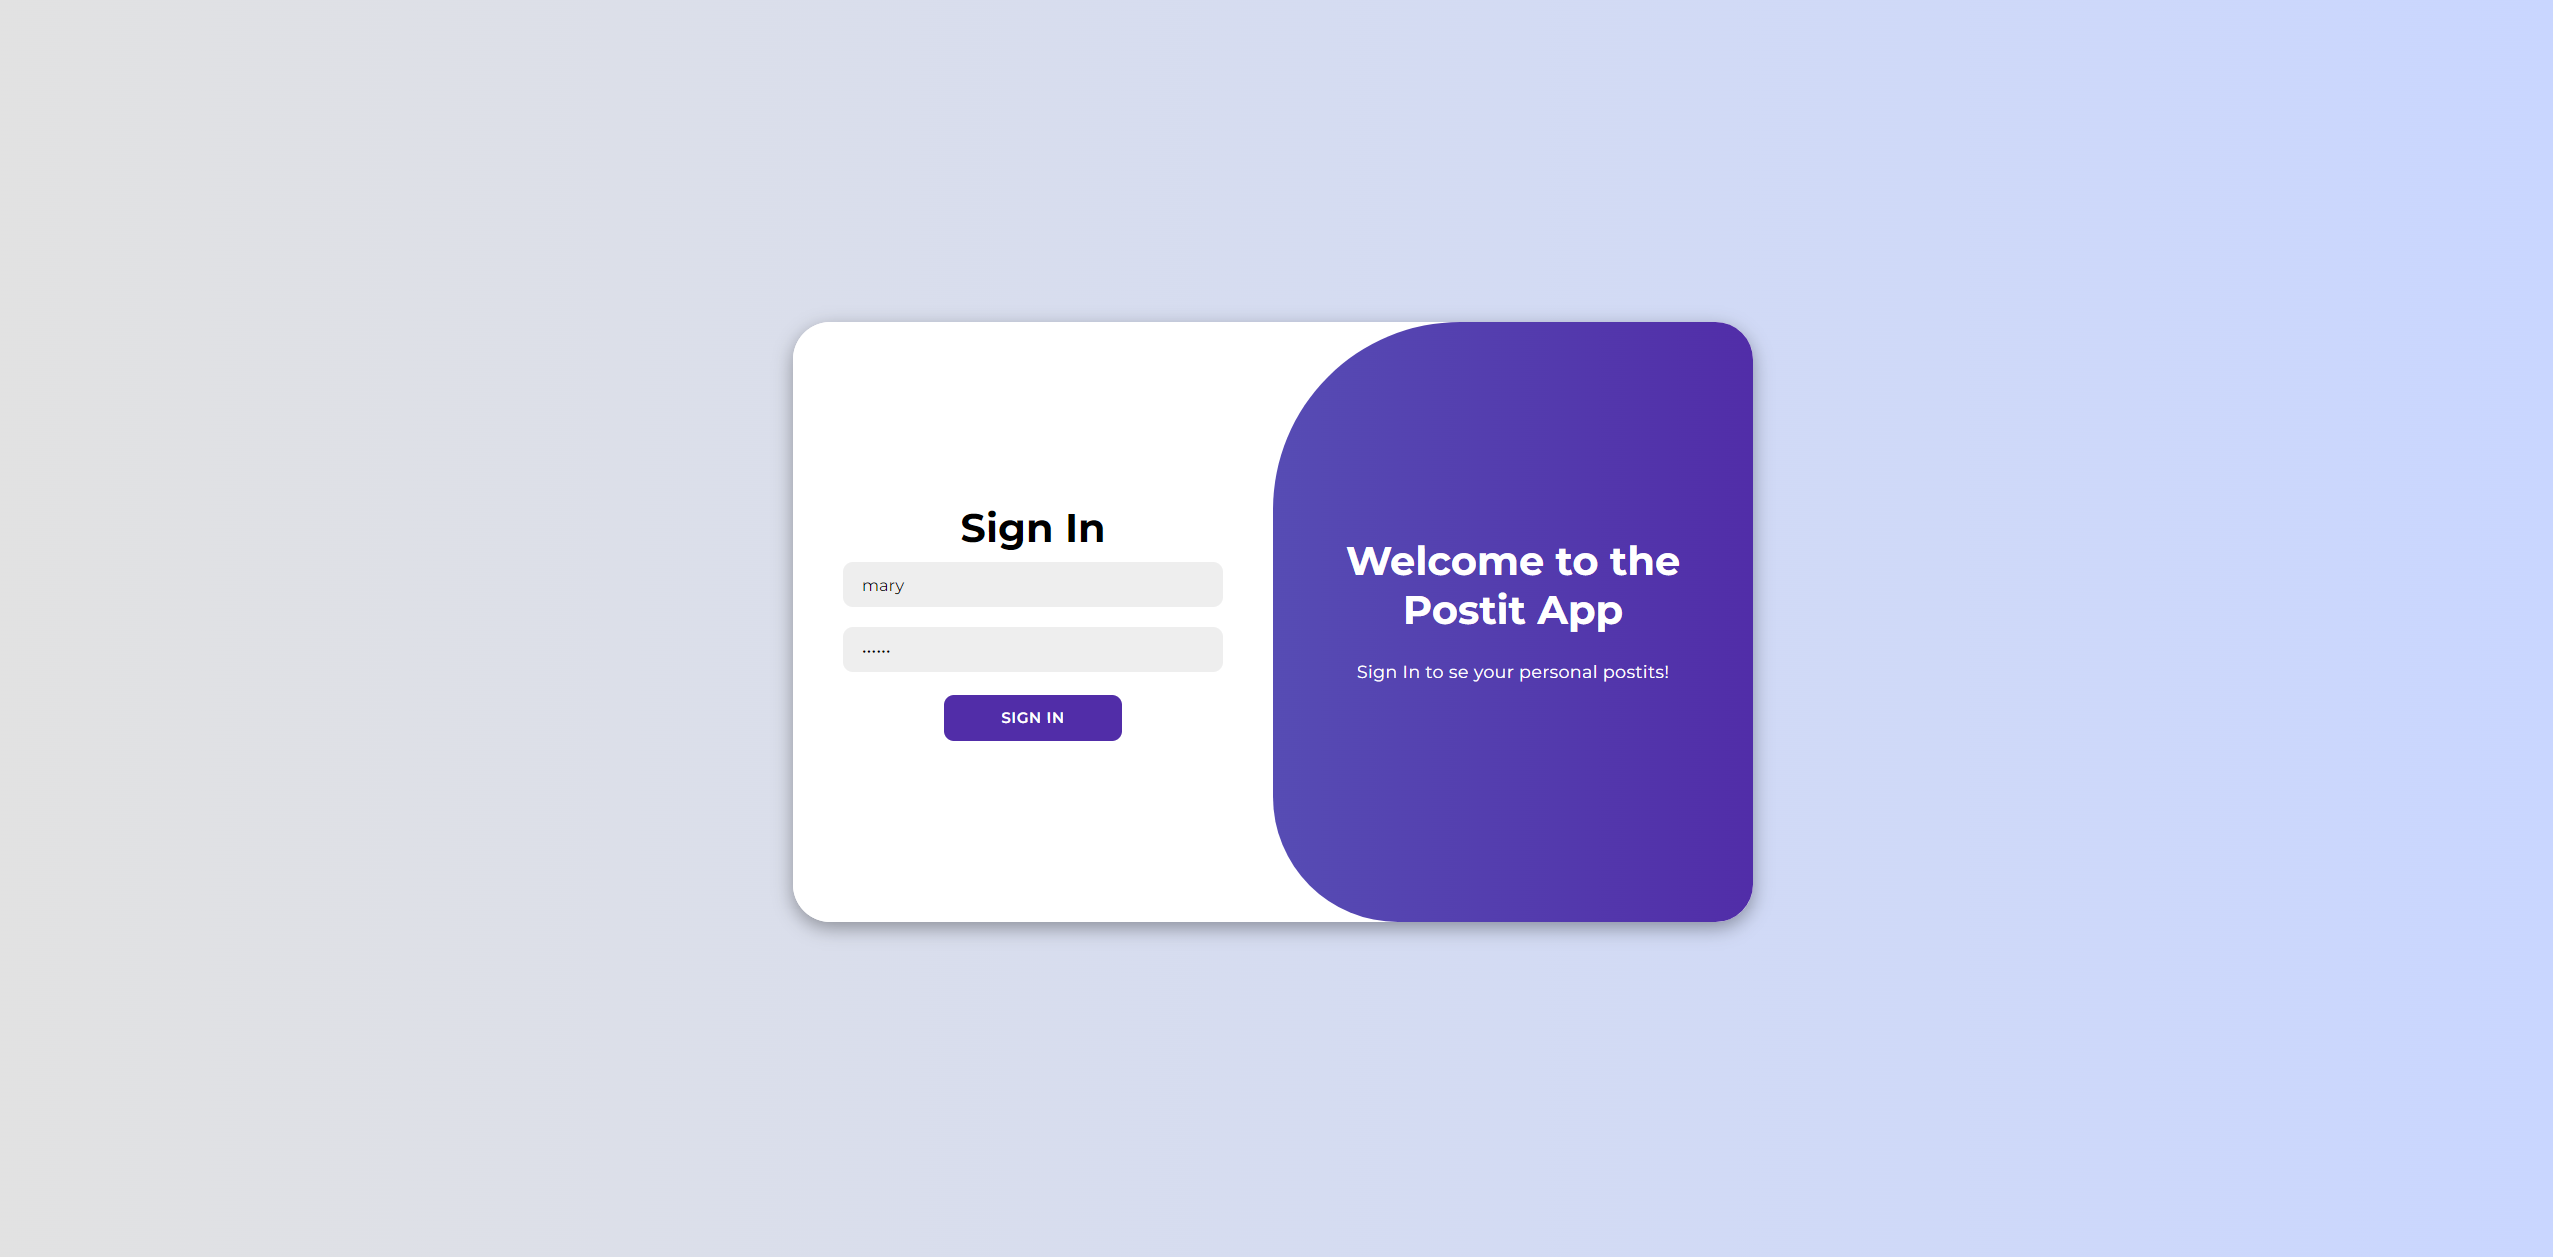
\includegraphics[width=0.9\textwidth]{images/1 login.png}
        \caption{Pagina di login}
         \subsubsection{Visualizza la homepage}
        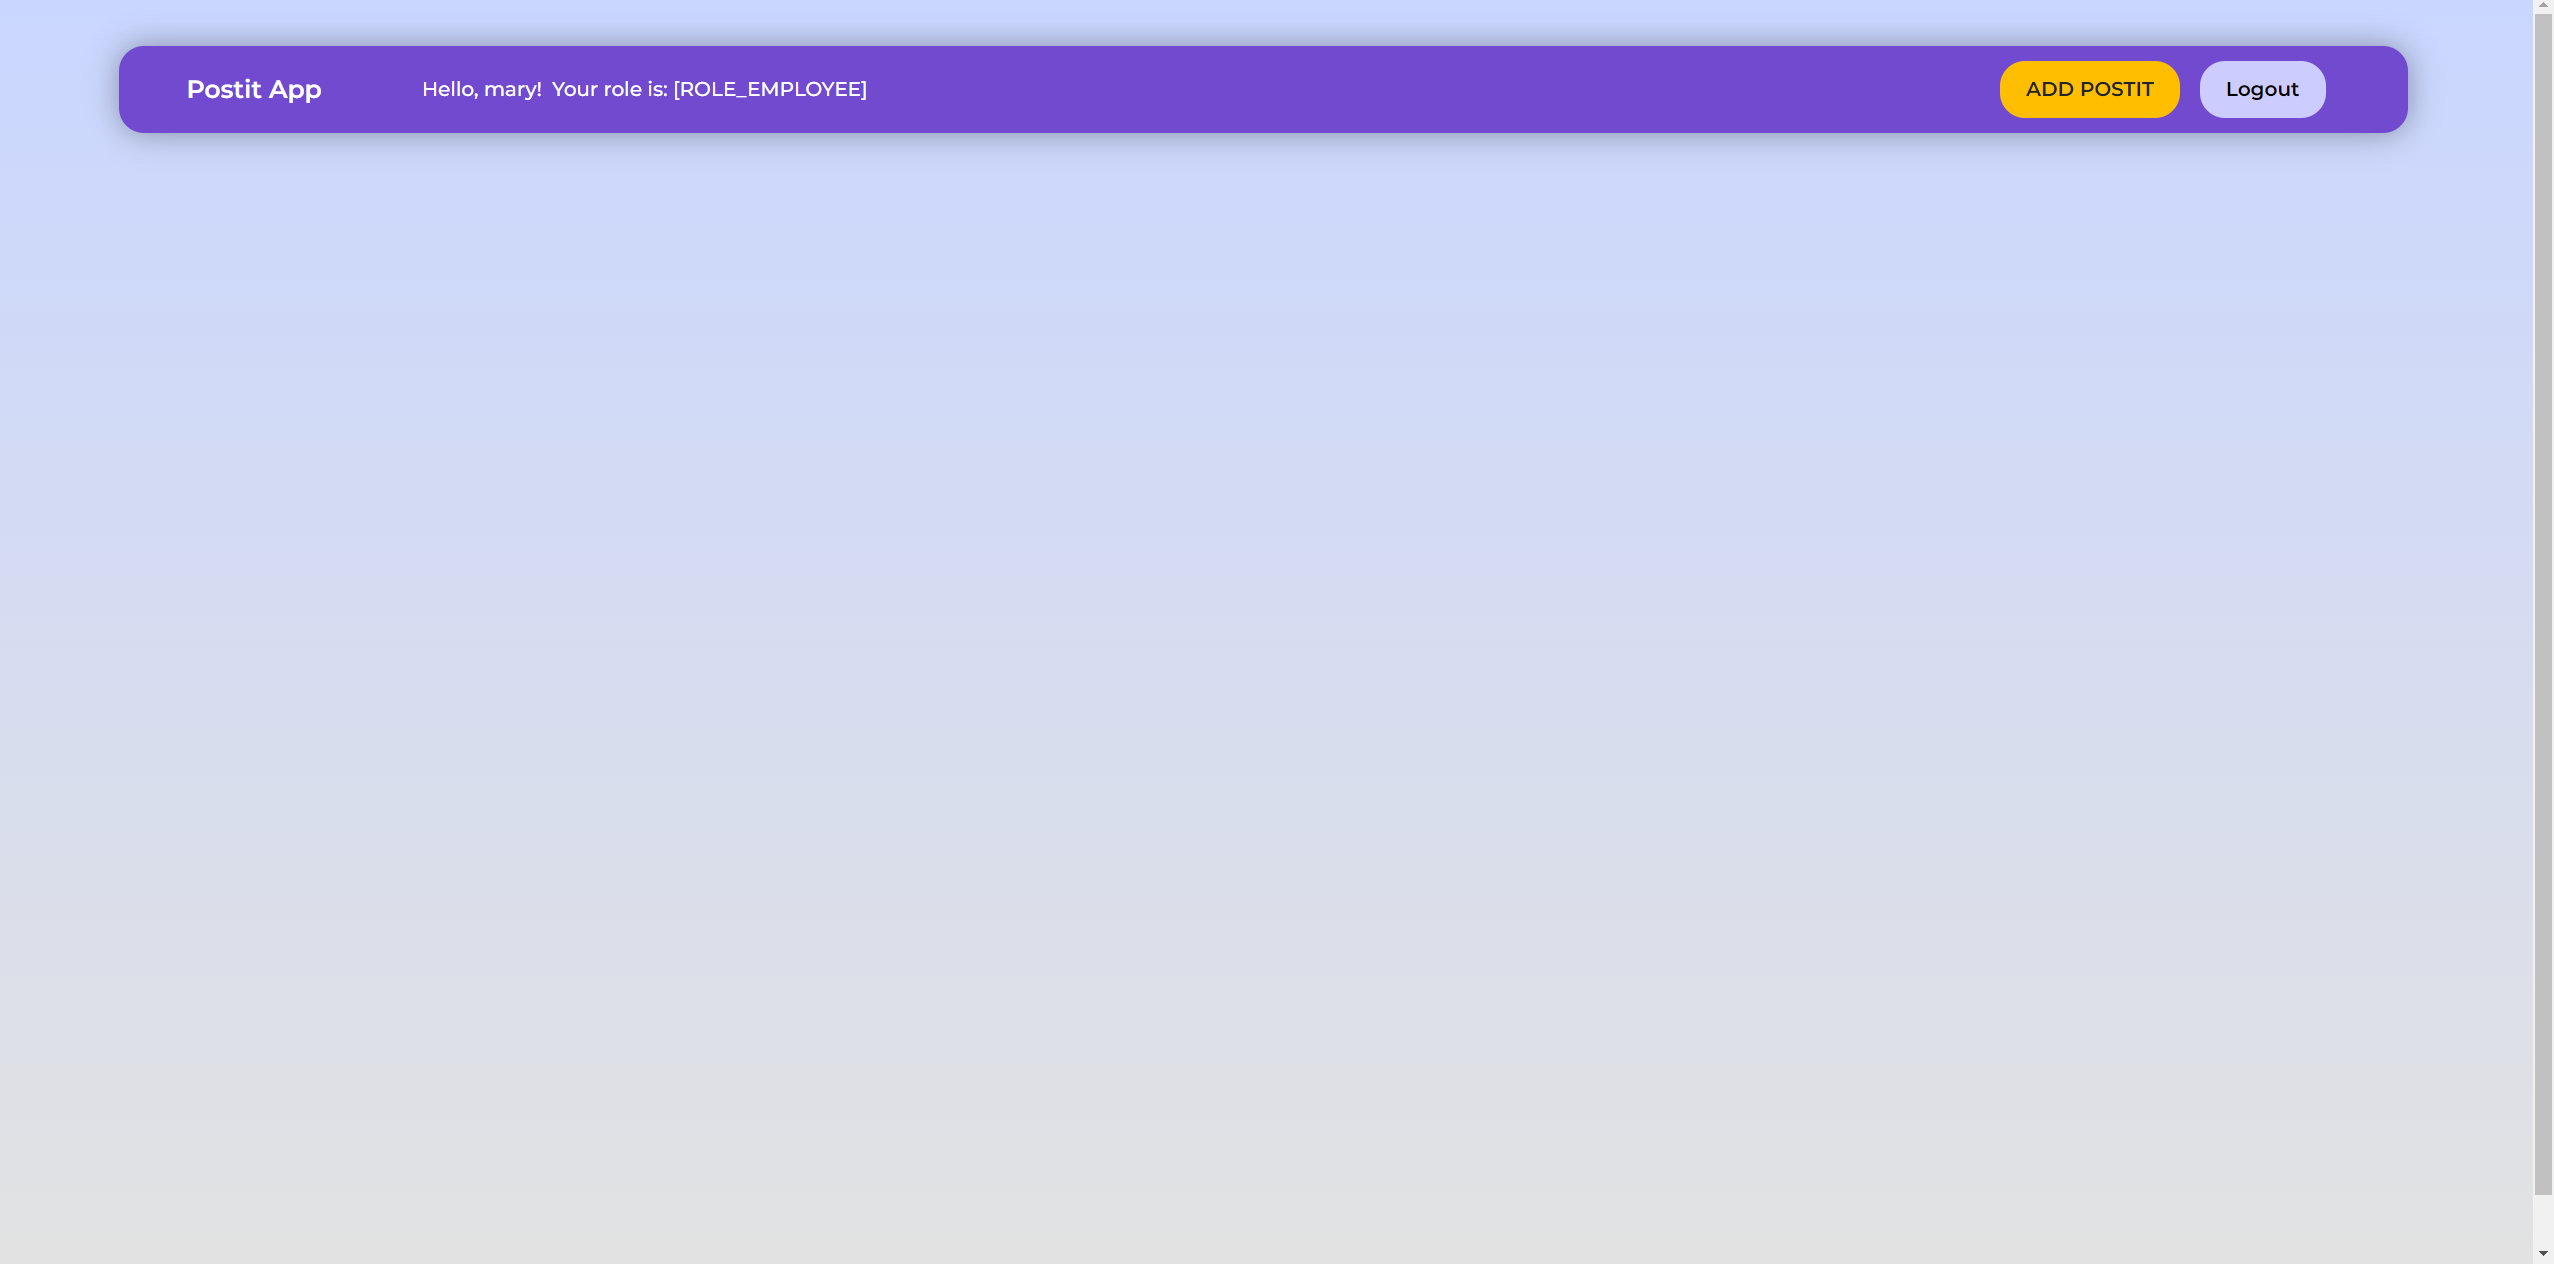
\includegraphics[width=0.9\textwidth]{images/2 homepage vuota.png}
        \caption{Home page}
        \label{fig:enter-label}
    \end{figure}
\end{center}
\vspace*{\fill}

\newpage

\vspace*{\fill}
\begin{center}
    \begin{figure}[h]
        \centering
        \subsubsection{Aggiunge 3 postit}
        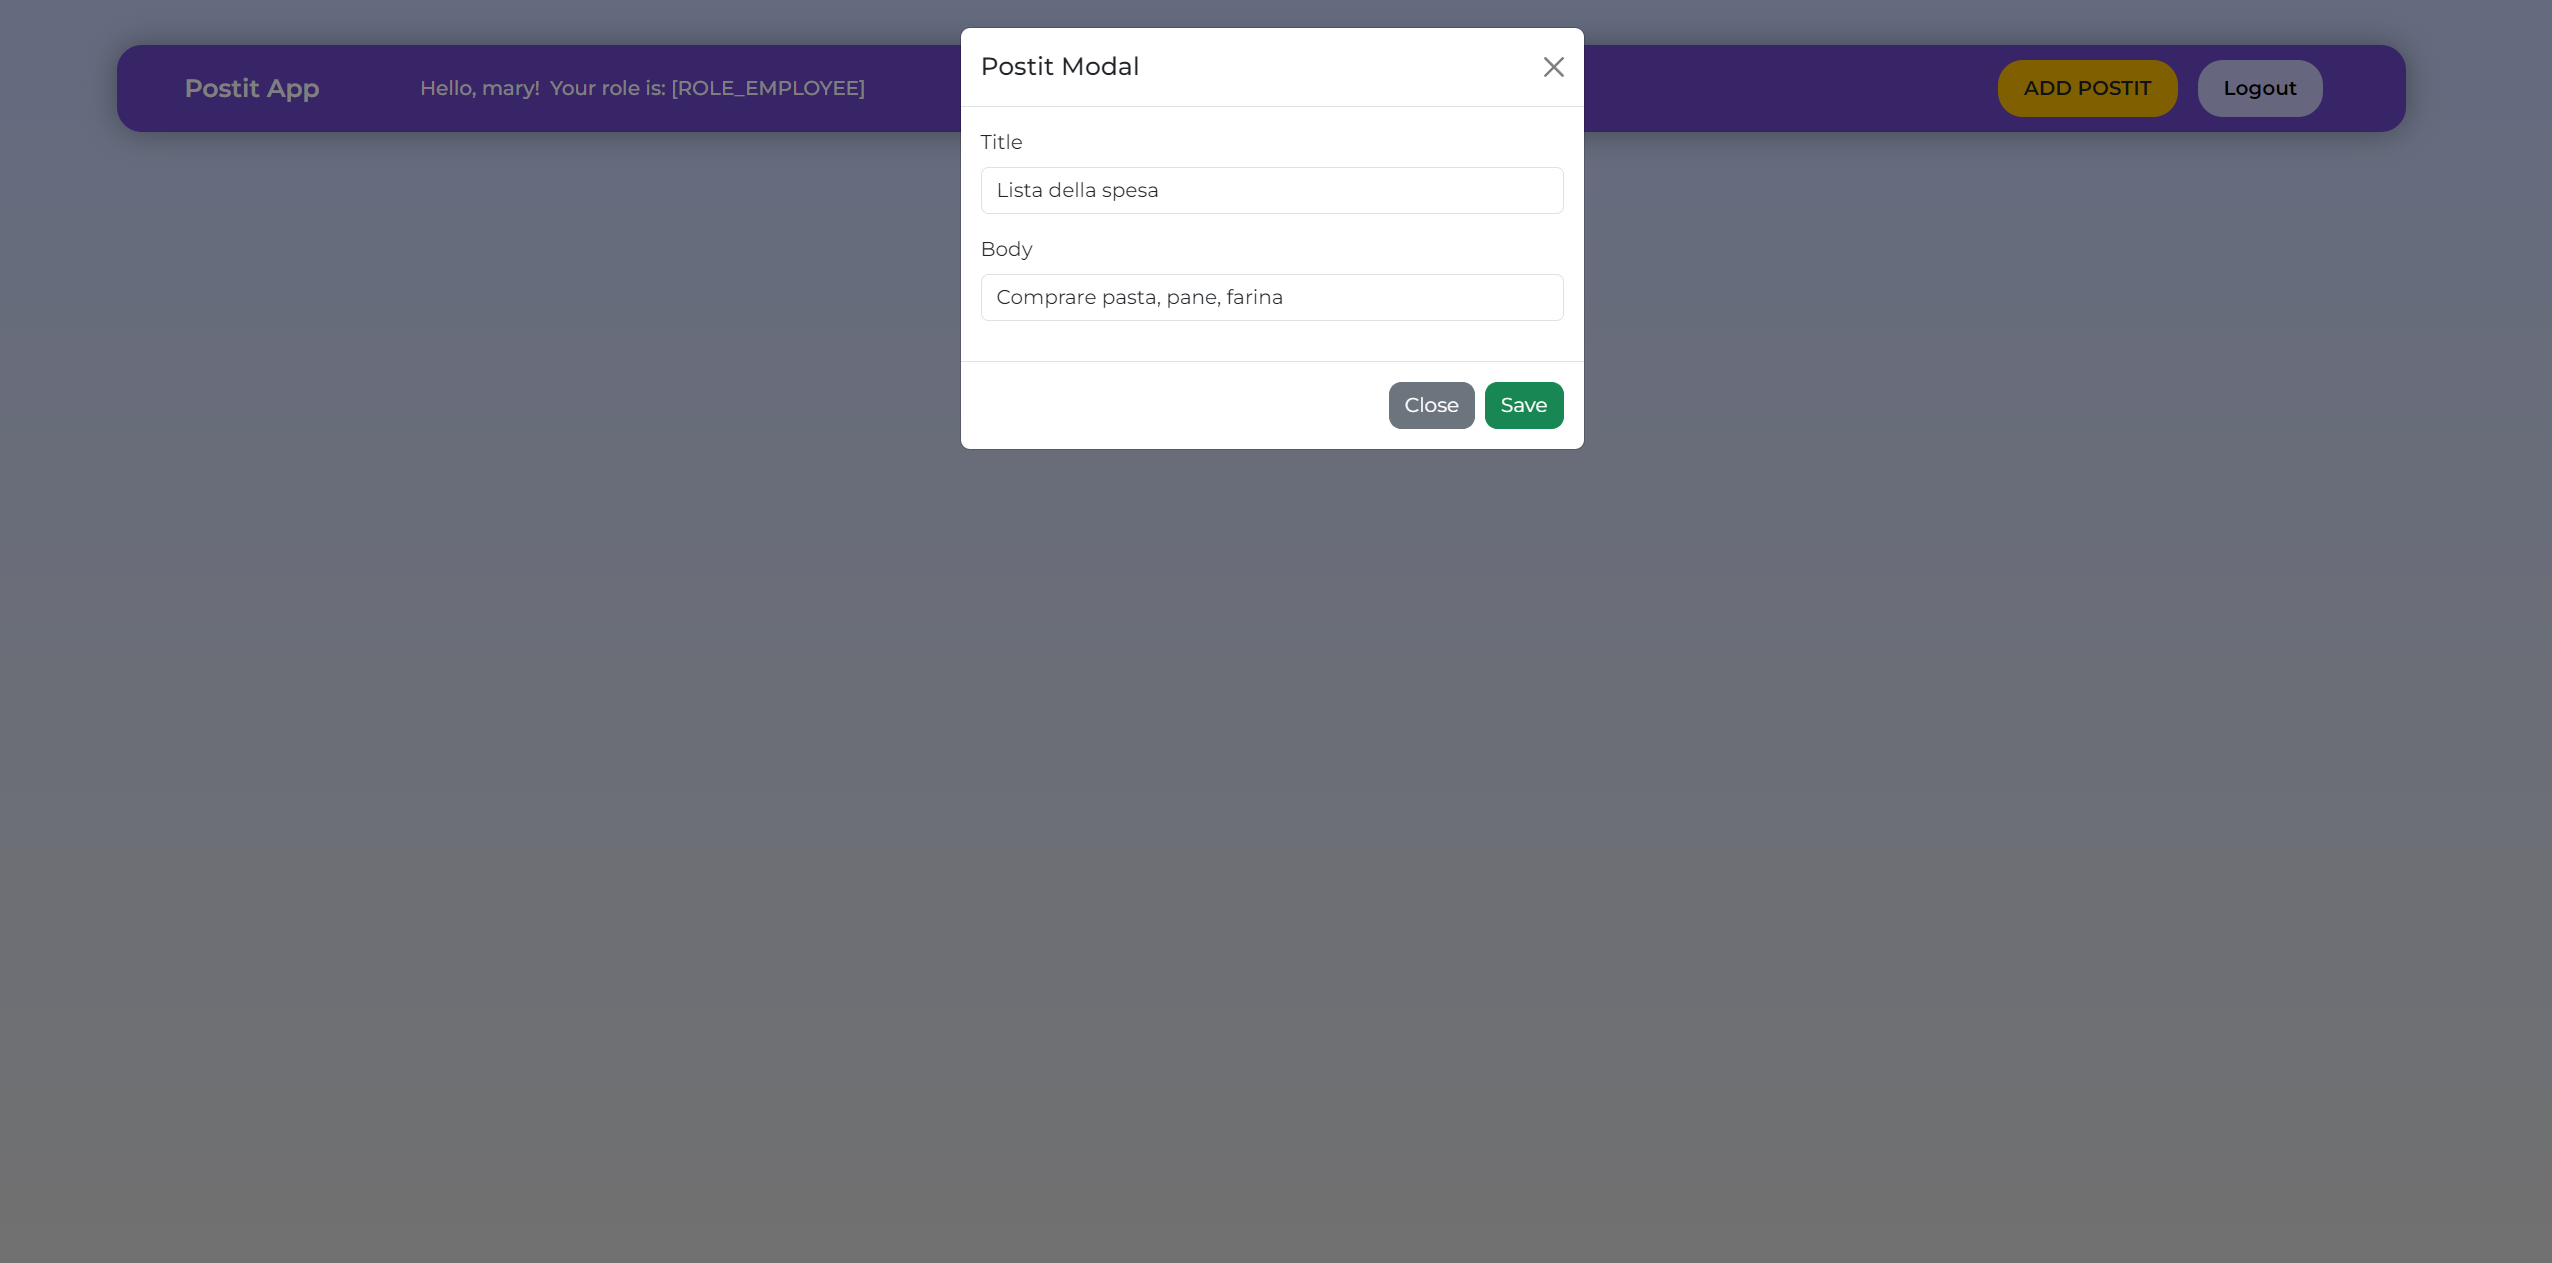
\includegraphics[width=0.9\textwidth]{images/3 aggiunta postit.png}
        \caption{Modal creazione postit}
         \subsubsection{Visualizza nella homepage i postit creati}
        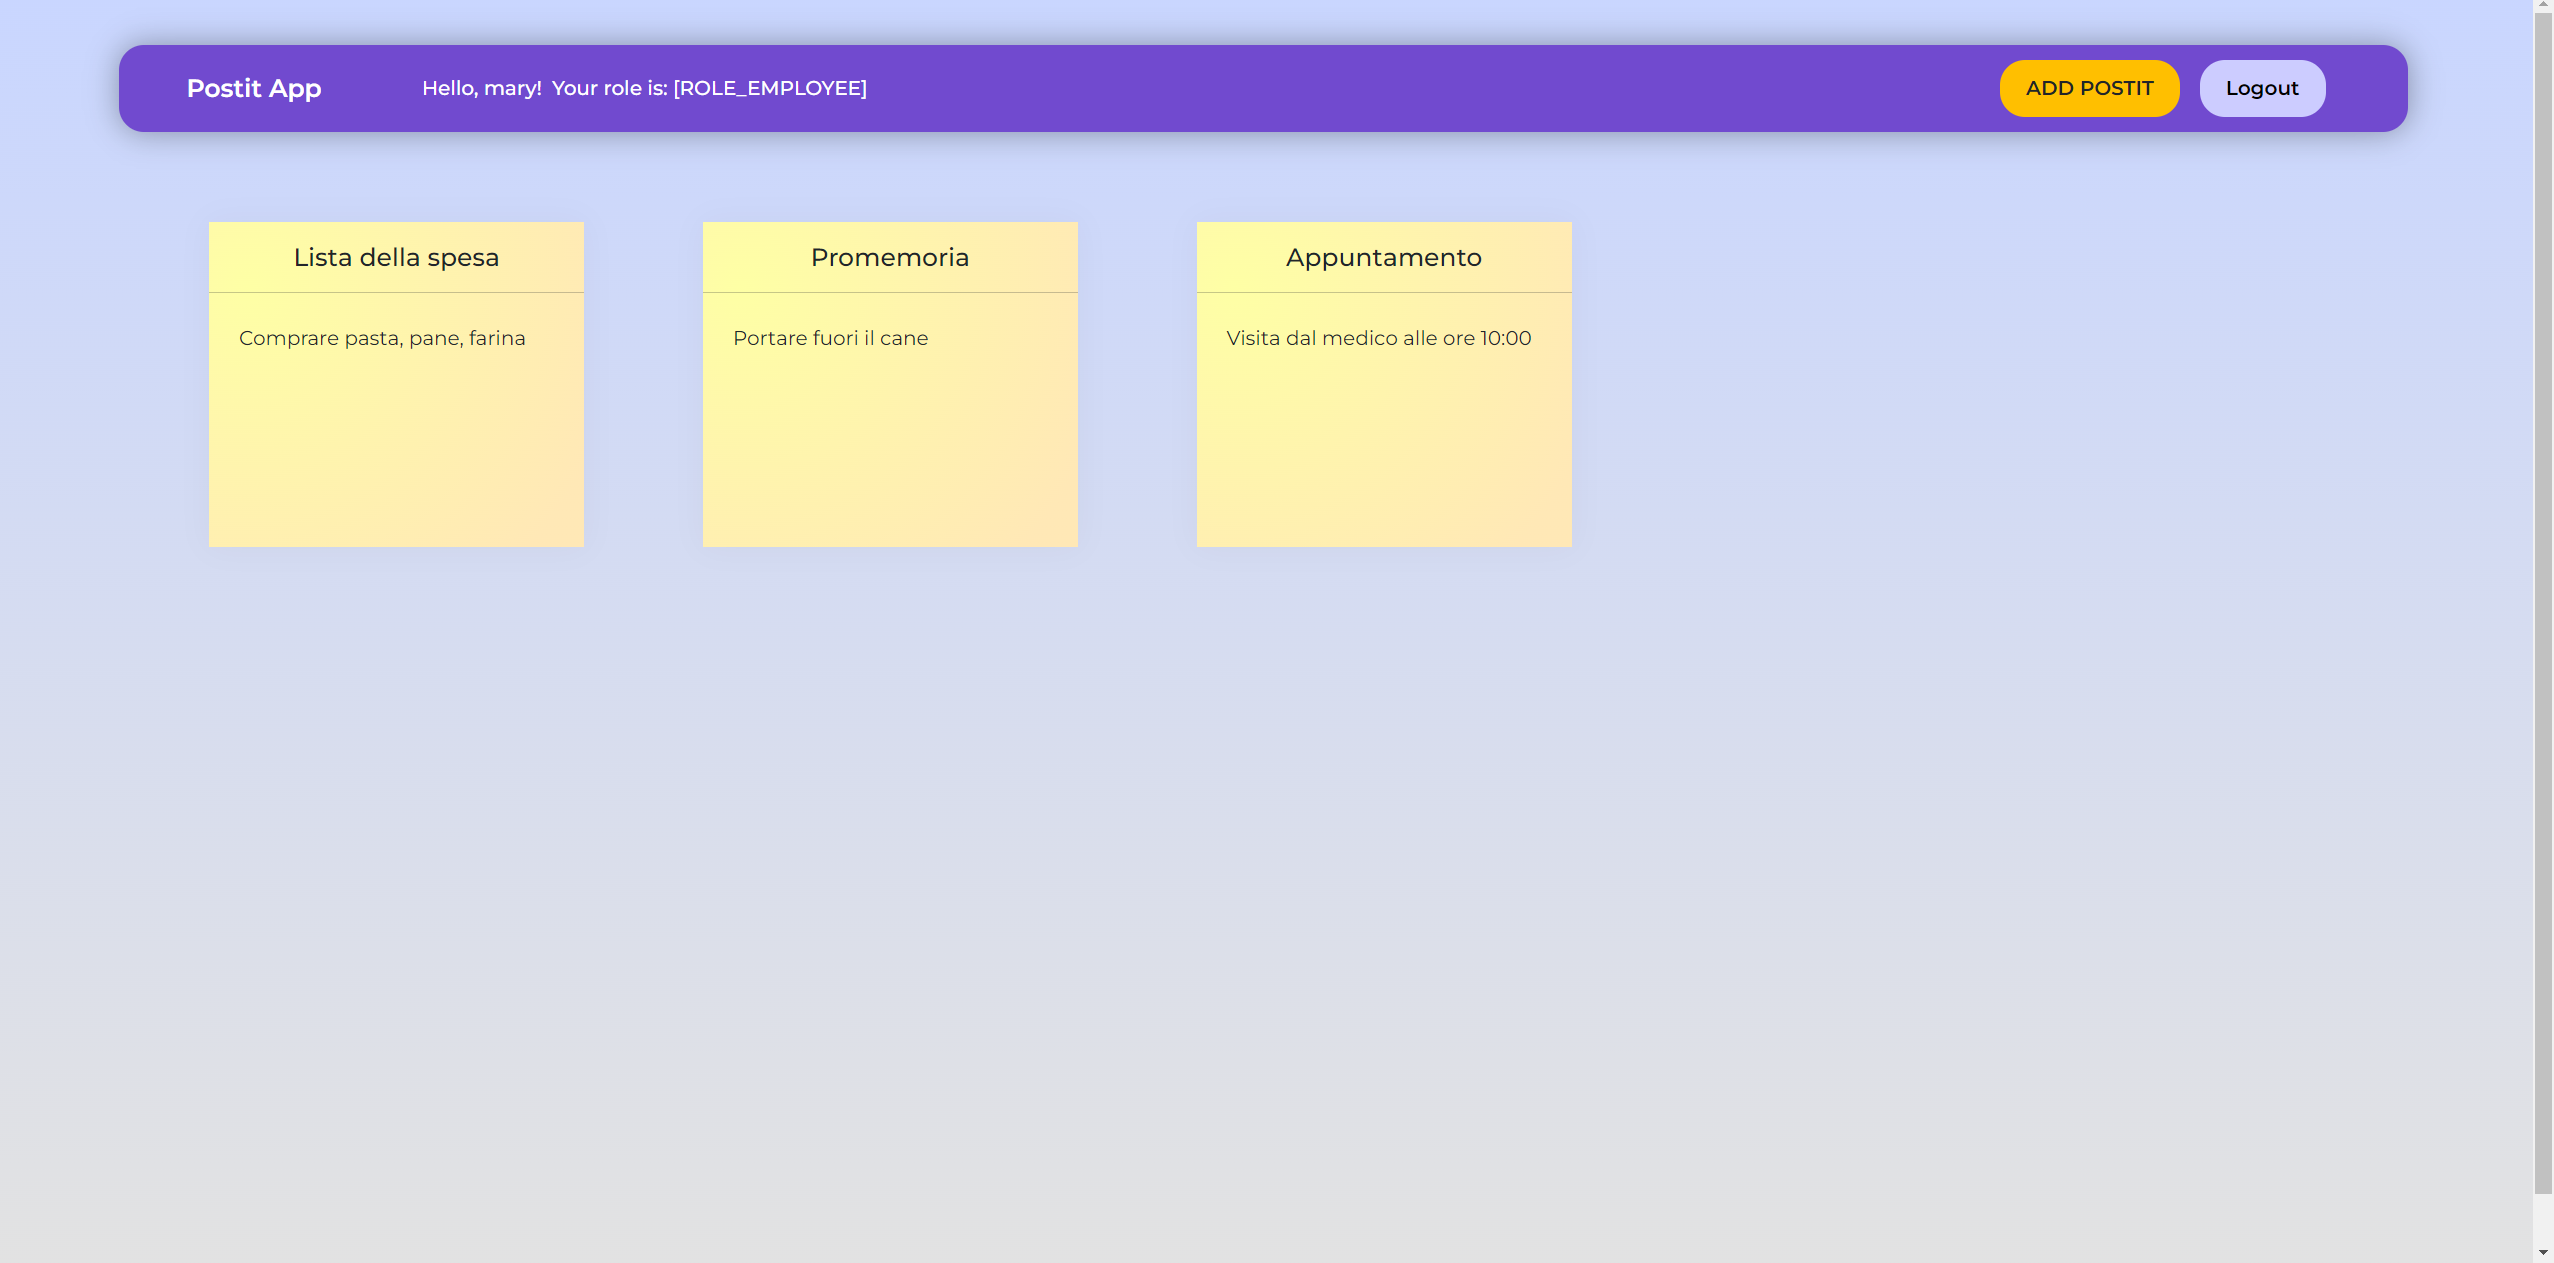
\includegraphics[width=0.9\textwidth]{images/4 postit visualizzati.png}
        \caption{Homepage che visualizza i 3 postit creati}
        \label{fig:enter-label}
    \end{figure}
\end{center}
\vspace*{\fill}

\newpage

\vspace*{\fill}
\begin{center}
    \begin{figure}[h]
        \centering
        \subsubsection{Modifica il primo postit}
        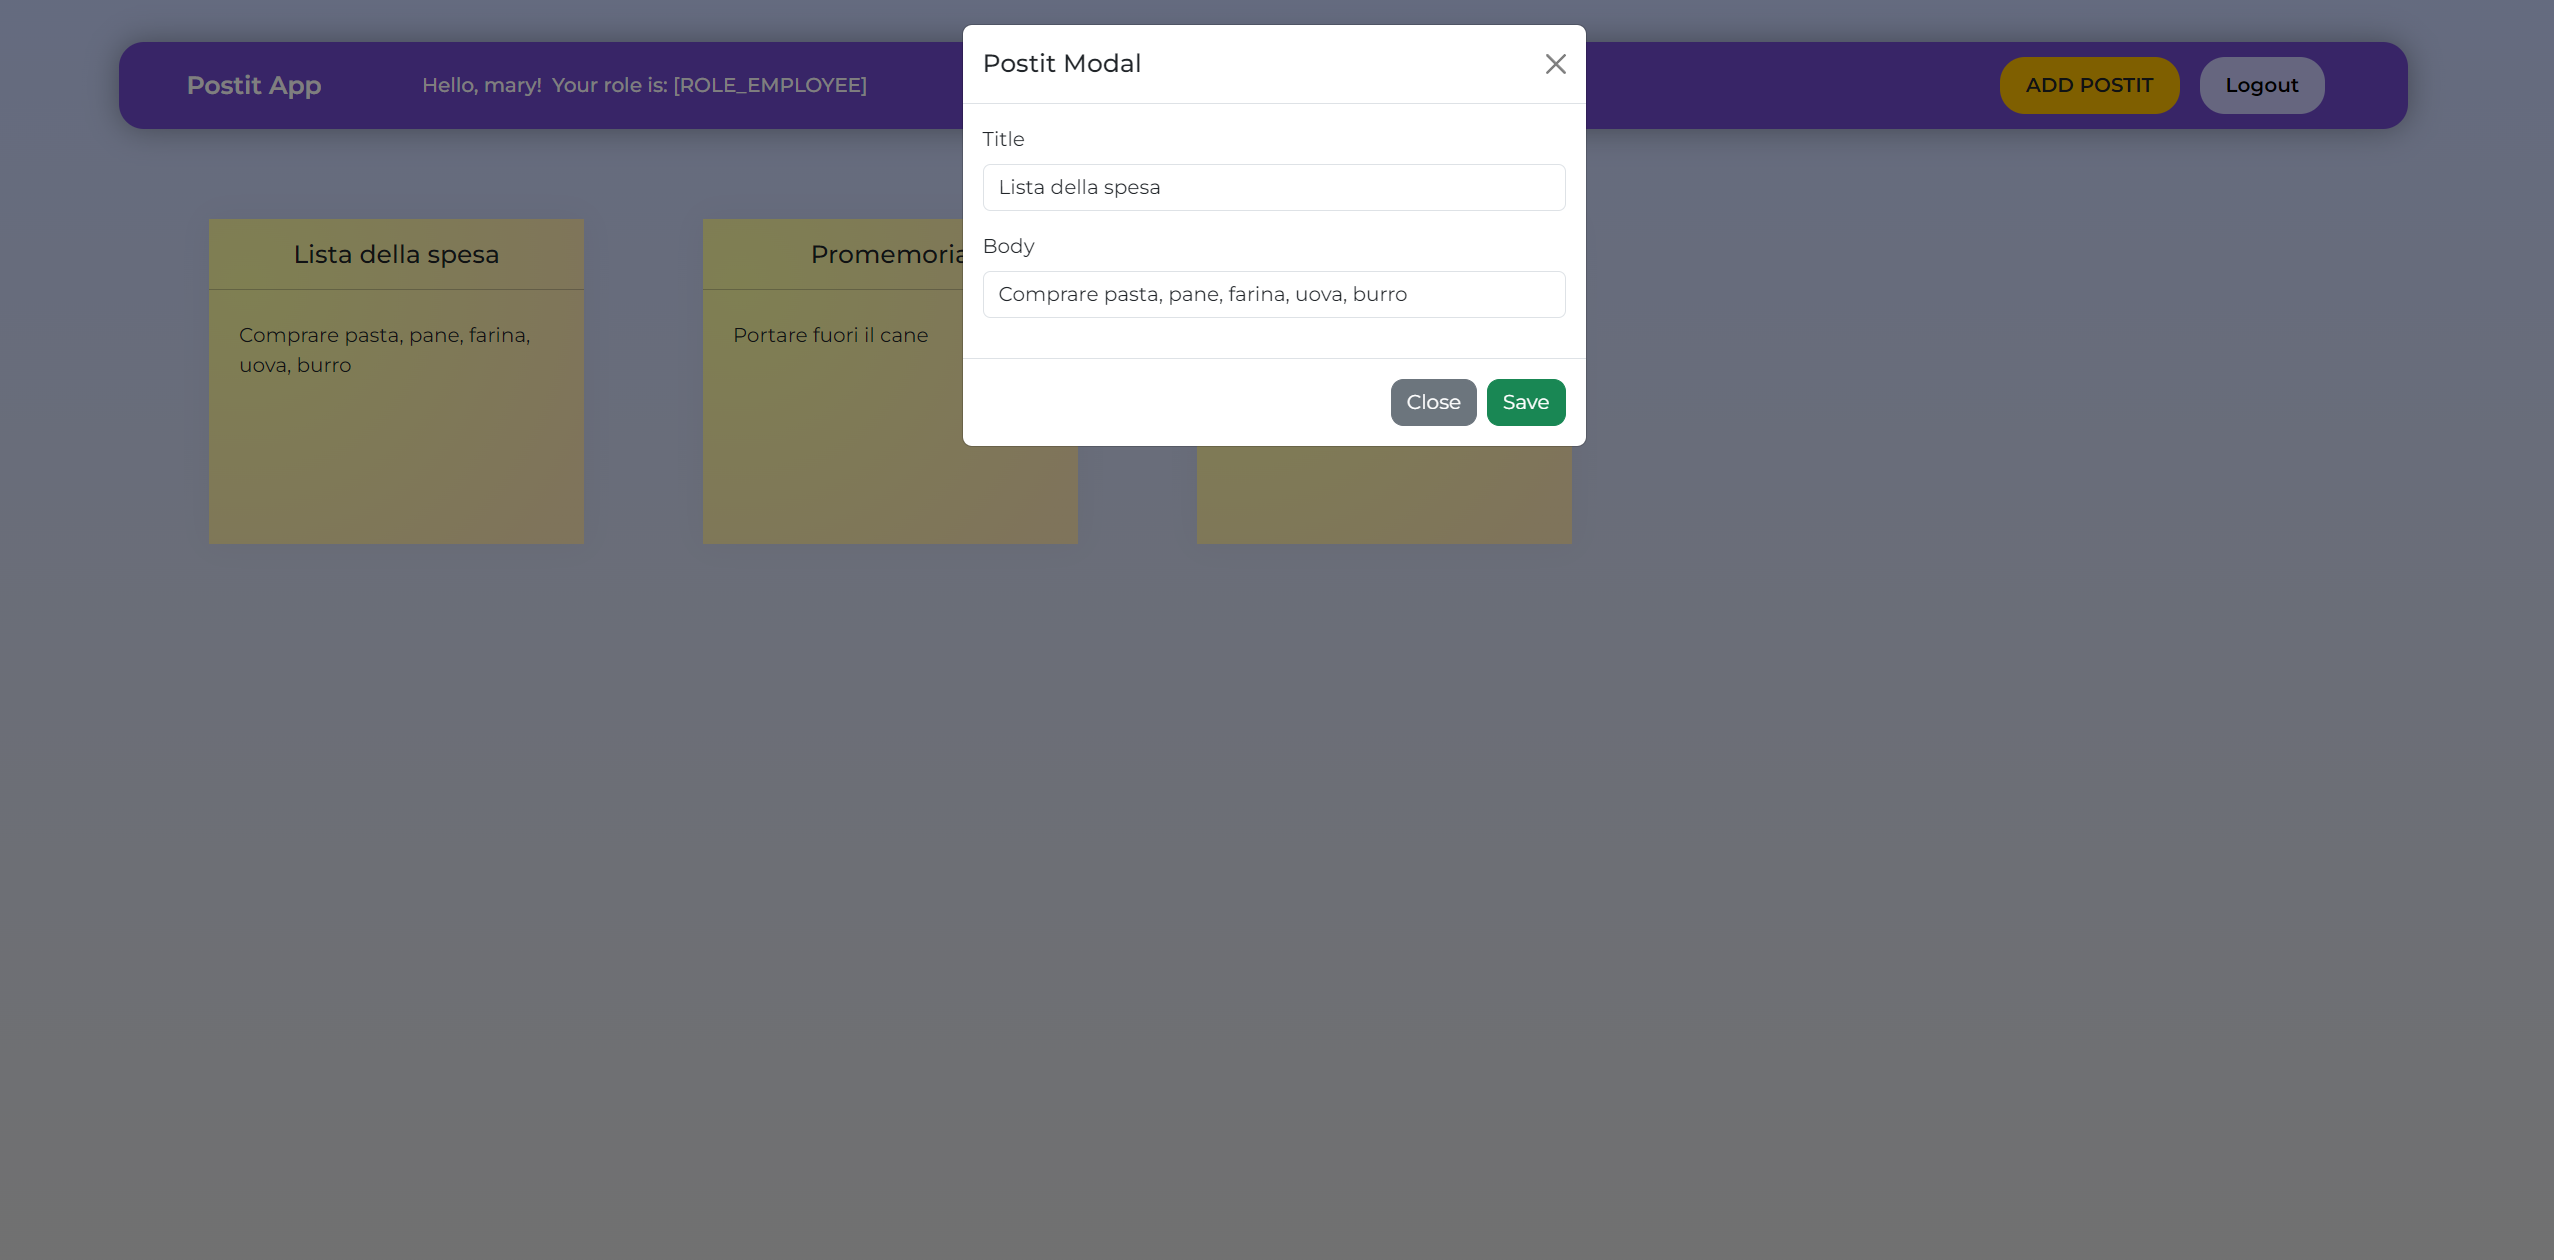
\includegraphics[width=0.9\textwidth]{images/5 modifica postit.png}
        \caption{Modal di modifica postit}
         \subsubsection{Elimina l'ultimo postit}
        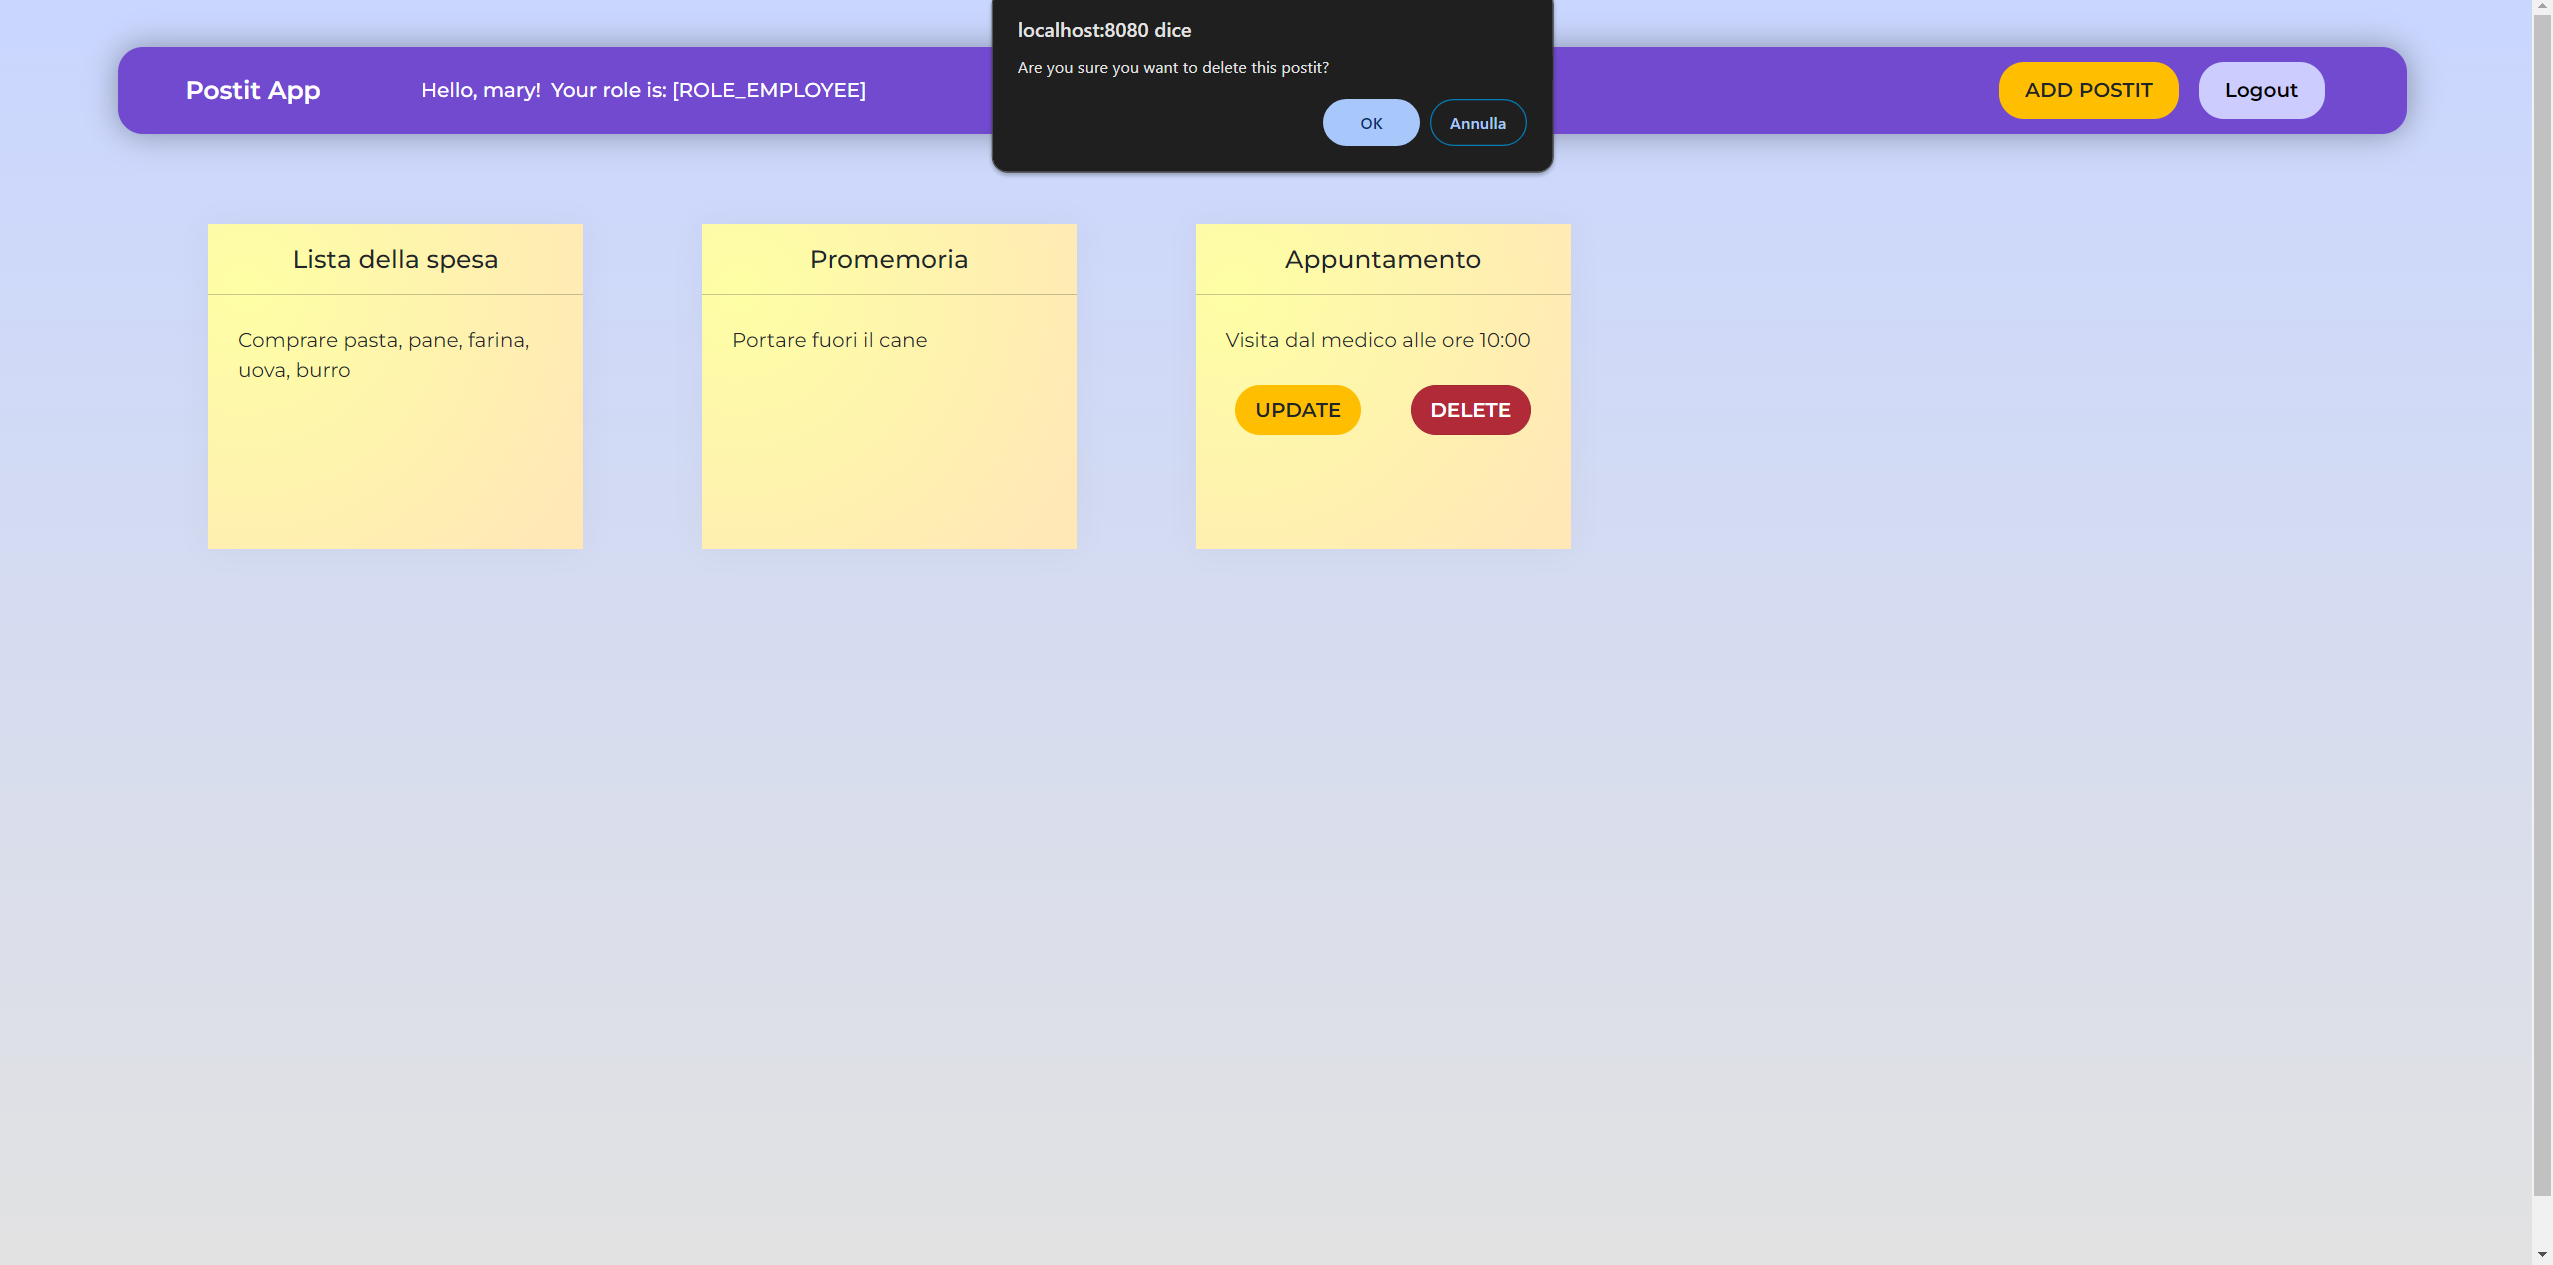
\includegraphics[width=0.9\textwidth]{images/6 eliminazione postit.png}
        \caption{Alert di eliminazione postit}
        \label{fig:enter-label}
    \end{figure}
\end{center}
\vspace*{\fill}

\newpage

\begin{center}
    \begin{figure}[th]
        \centering
        \subsubsection{Effettua il logout}
        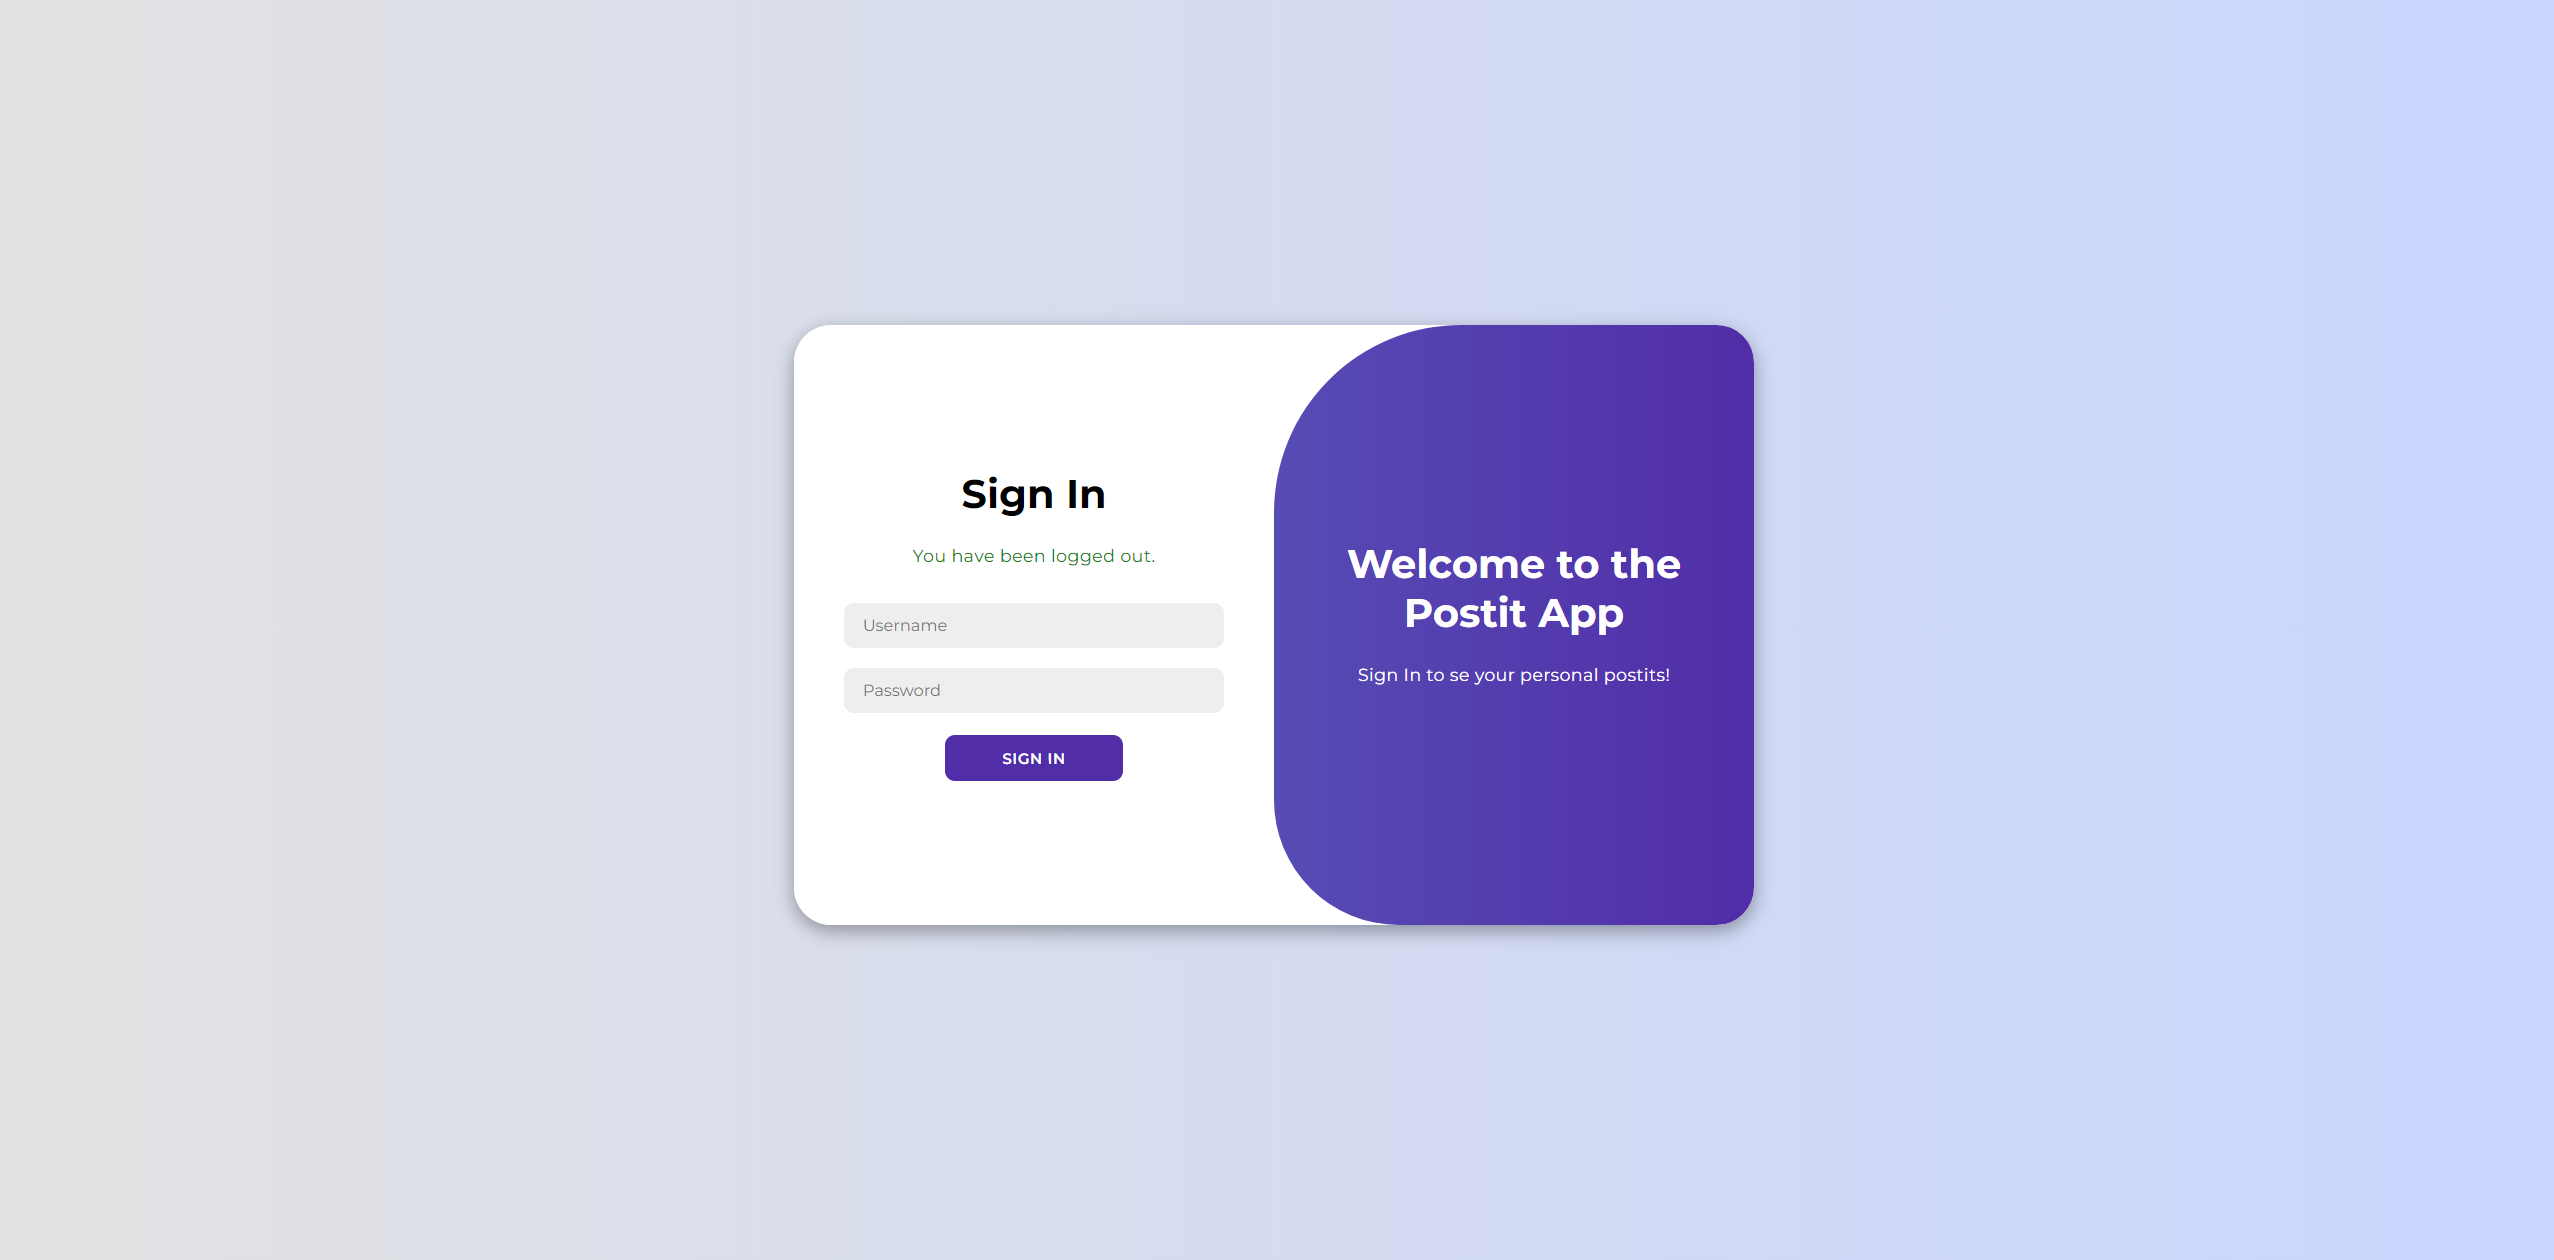
\includegraphics[width=0.9\textwidth]{images/7 logout.png}
        \caption{Pagina di login dopo aver effettuato il logout}
        \label{fig:enter-label}
    \end{figure}
\end{center}
\vspace*{\fill}

\cleardoublepage
\renewcommand{\headrulewidth}{0pt}
\rhead{}
\thispagestyle{plain}
\begingroup
\let\clearpage\endgroup
\null\vspace{\stretch{1}}

\chapter*{\centering Postfazione}
\addcontentsline{toc}{chapter}{Postfazione}
Lavorare a questa tesi mi ha permesso di esplorare il mondo dello sviluppo web affrontando temi come la progettazione di una web app con la sua relativa struttura, composta da back-end e front-end, approfondendo anche l'ambito della gestione dei dati attraverso l'utilizzo di un database.
L'impegno nello sviluppo di questo progetto si è rivelato fondamentale per comprendere le tecnologie utilizzate nello sviluppo di web app al giorno d'oggi, espandendo le mie conoscenze e capacità nel sapermi approcciare a tecnologie diverse da quelle che ho visto fino ad ora.

Ci tengo a ringraziare il mio relatore per tutte le linee guida e consigli che mi ha fornito, al fine di rendere la scrittura di questa tesi possibile.


\vspace{\stretch{2}} \null
\clearpage
\renewcommand{\headrulewidth}{0pt}
\thispagestyle{plain}
\rhead{}

\backmatter


\bibliographystyle{unsrtnat}
\bibliography{bibliografia}

\end{document}

% per citare la bibliografia faccio: \cite{aniba2008knowledge}
%\myemptypage
%\hspace{1em} % per aggiungere una linea vuota spazio